\documentclass[english]{article}
\usepackage[T1]{fontenc}
\usepackage[latin9]{inputenc}
\usepackage{babel}
\usepackage{graphicx}
\usepackage{subfigure}
\usepackage{float}
\setlength{\parindent}{0pt}

\begin{document}

\title{Lab 6: 3D Inspection\\ -------------------------------- \\ \Large Sensors and Digitization}
\author{ \ Armine Vardazaryan, Songyou Peng \\ arminevardazaryan@gmail.com, psy920710@gmail.com}
\date{9th November 2015}

\maketitle

\section*{Introduction}
The objective of this lab work is to conduct 3D inspection with a compact vision system. The system used is based on a high-accuracy Laser Displacement Sensor.
This kind of sensor can be used in measurements of heights at multiple points, width/gap on the surface profile, section area, intersections/angle measurements, etc. The Laser sensor head is able to measure surface profile of targets in X and Z directions. The height, width or gap on a surface profile can be measured using 28 measurement modes[1].
Measuring range for the sensor head is 200$\pm$48 mm.

\section*{Equipment and the setup}
In this experiment we used the KEYENCE LJ-G 080 high-accuracy laser displacement sensor with its appropriate equipment and the provided software LJ-G Navigator.\\
In preparation to the experiment, one important thing is to adjust the distance between camera and object. Different objects have different proper distances to the camera, as the laser beam must be well focused on the object. \\

\section*{Step Measurement}
Once the height of the sensor is properly adjusted and the laser is focused a good profile of the used object is visible on the screen. To save the profile of the measured object, we go to "Master reg" part to register this profile. In order to measure the step height of an object, first, in the "OUT setting", measurement type should be changed to "Step" mode. And then we should put two regions of interest in the profile, one in the peak and the other in the valley that together represent the step. This can be seen from Figure \ref{fig:one}.\\

\begin{figure}[H]
	\centering
	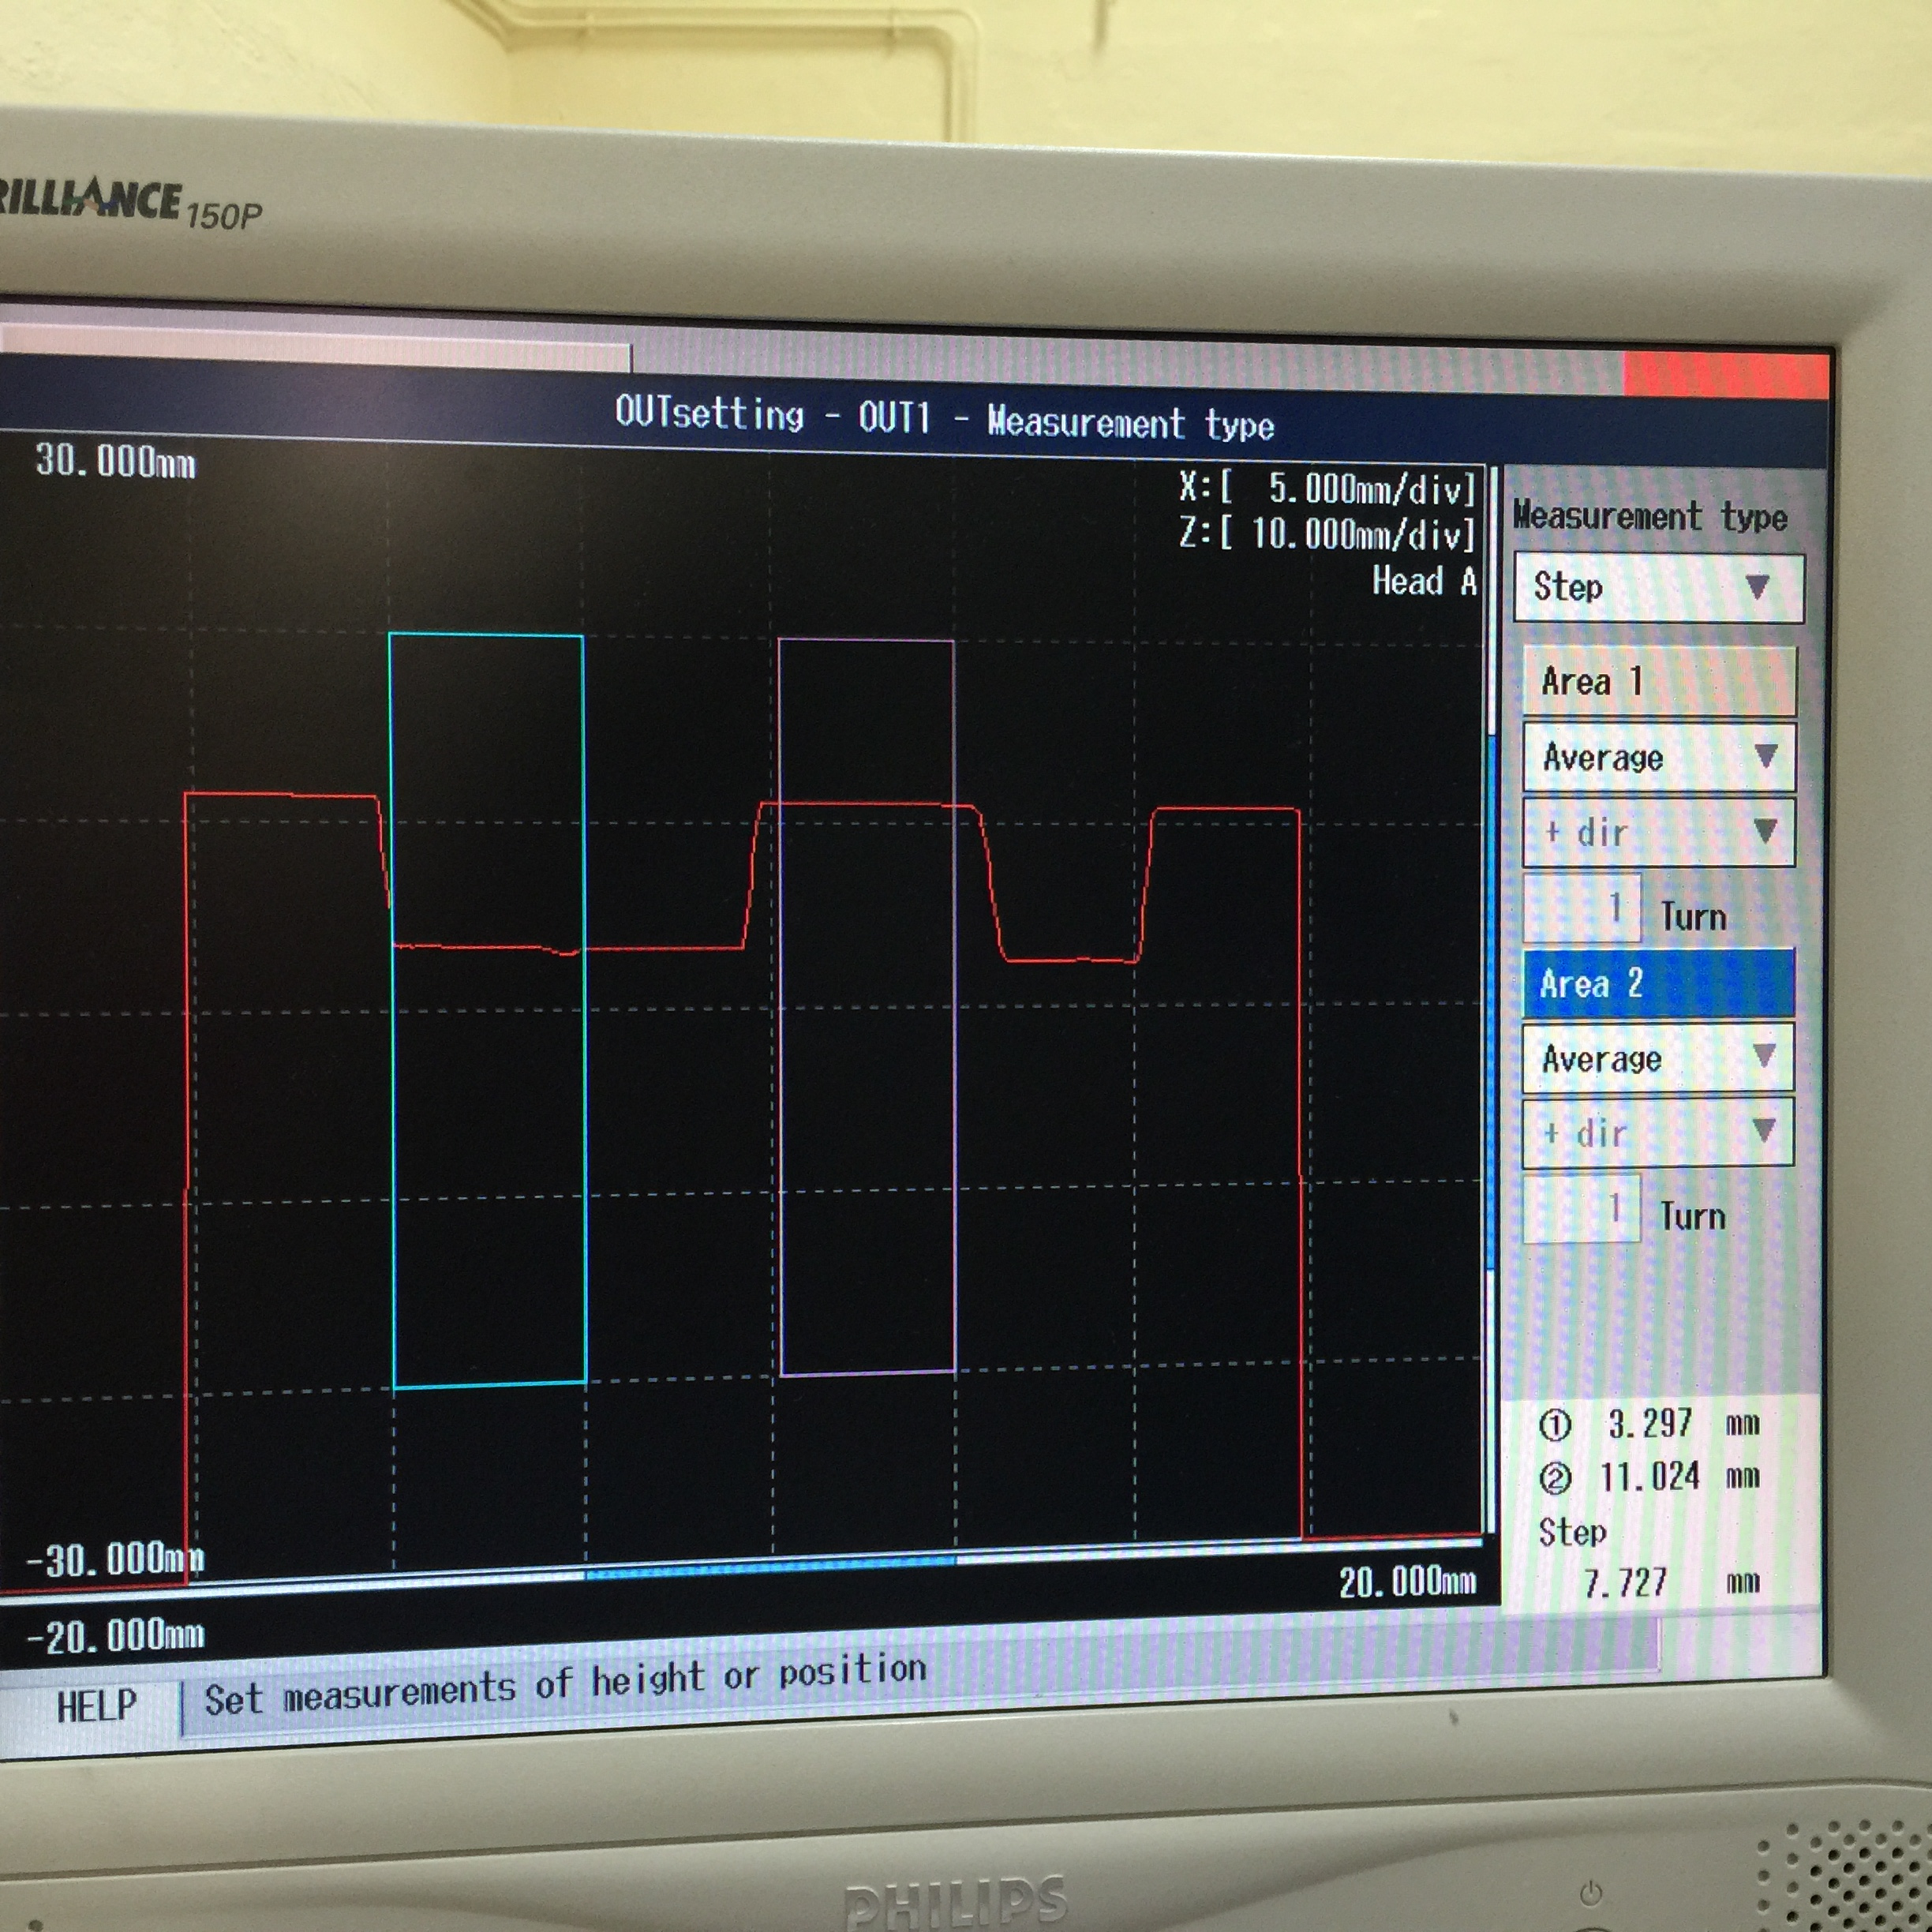
\includegraphics[width=0.8\linewidth]{Lab6/Step1.JPG}
	\caption{Set regions of interest in order to measure the height}
	\label{fig:one}
\end{figure}
The measurement result will be found by taking the difference in mean heights in the two specified regions. After the step is measured, we start to consider what if the object is shifted and angle is changed. So we perform shift and angle correction by setting region of moving in the tab "Pos Corr". The height measurement value in the top right side of Figure \ref{fig:twoa} and Figure \ref{fig:twob} show that accurate measured height could still be acquired even when the object is shifted or rotated.\\

\begin{figure}[H]
	\centering
	\subfigure[Original]{\label{fig:twoa}
	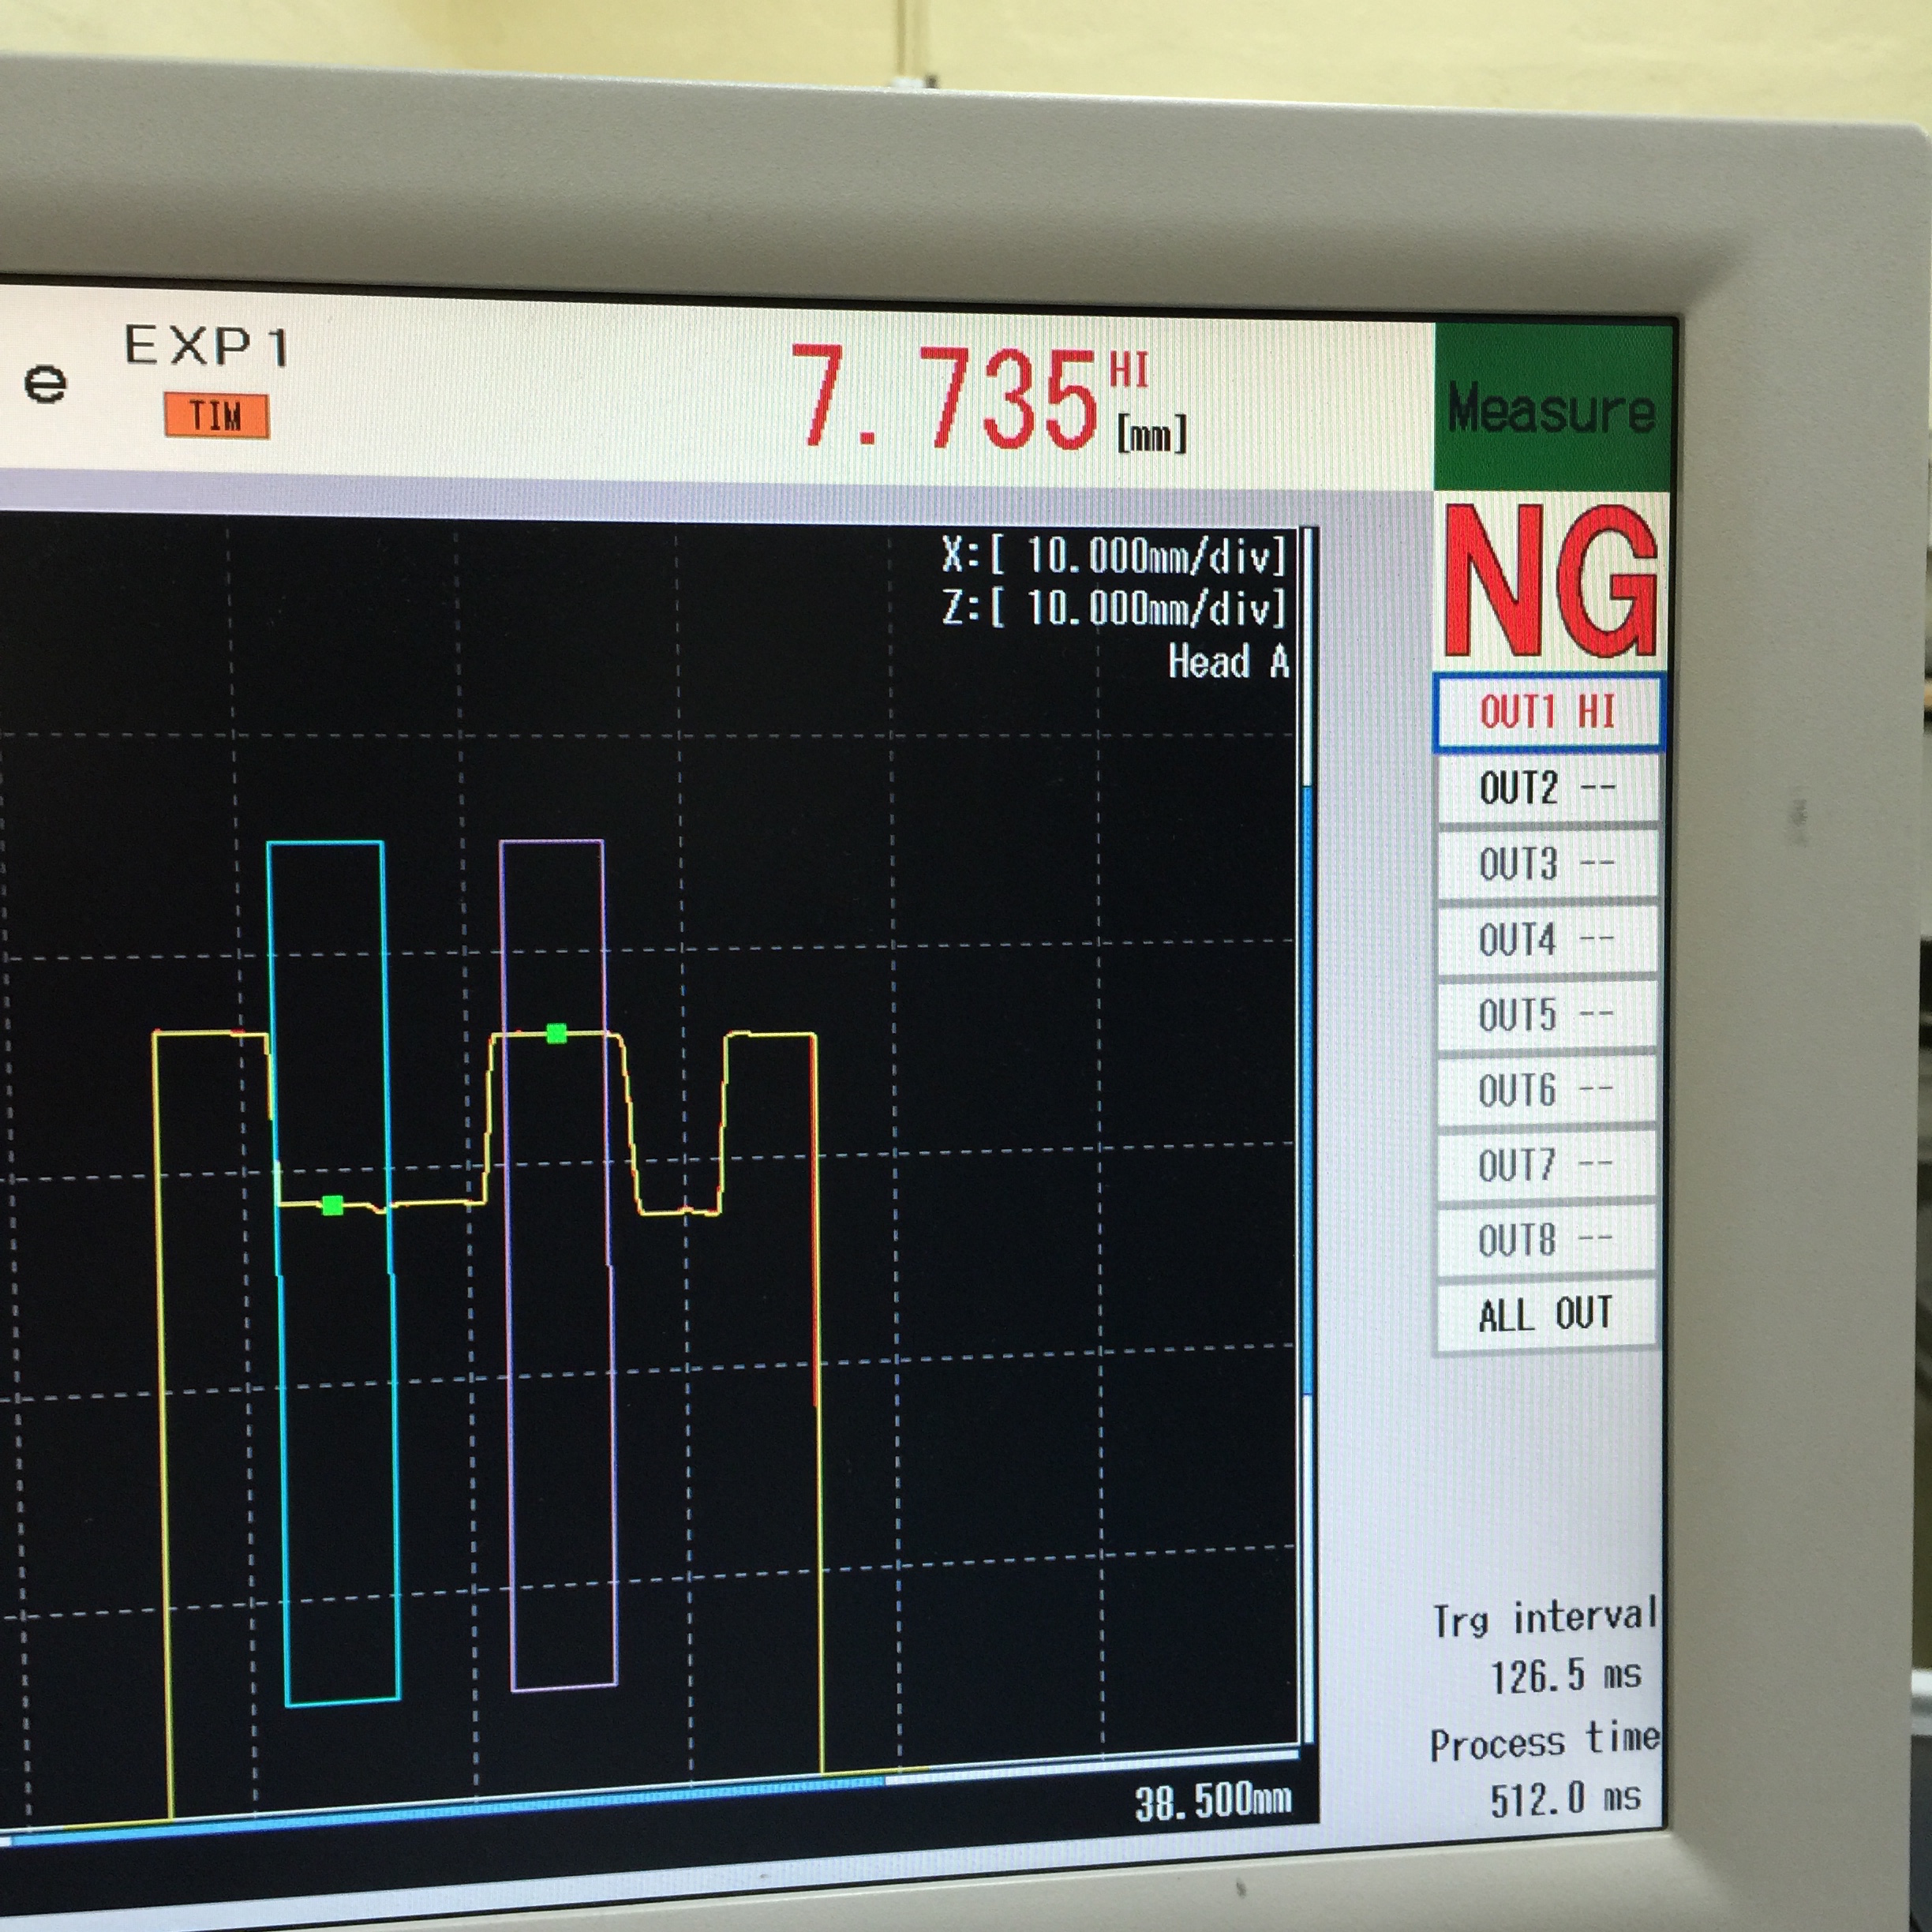
\includegraphics[width=0.4\linewidth]{Lab6/Step2.JPG}
	}
	\subfigure[Shift and Angle]{\label{fig:twob}
	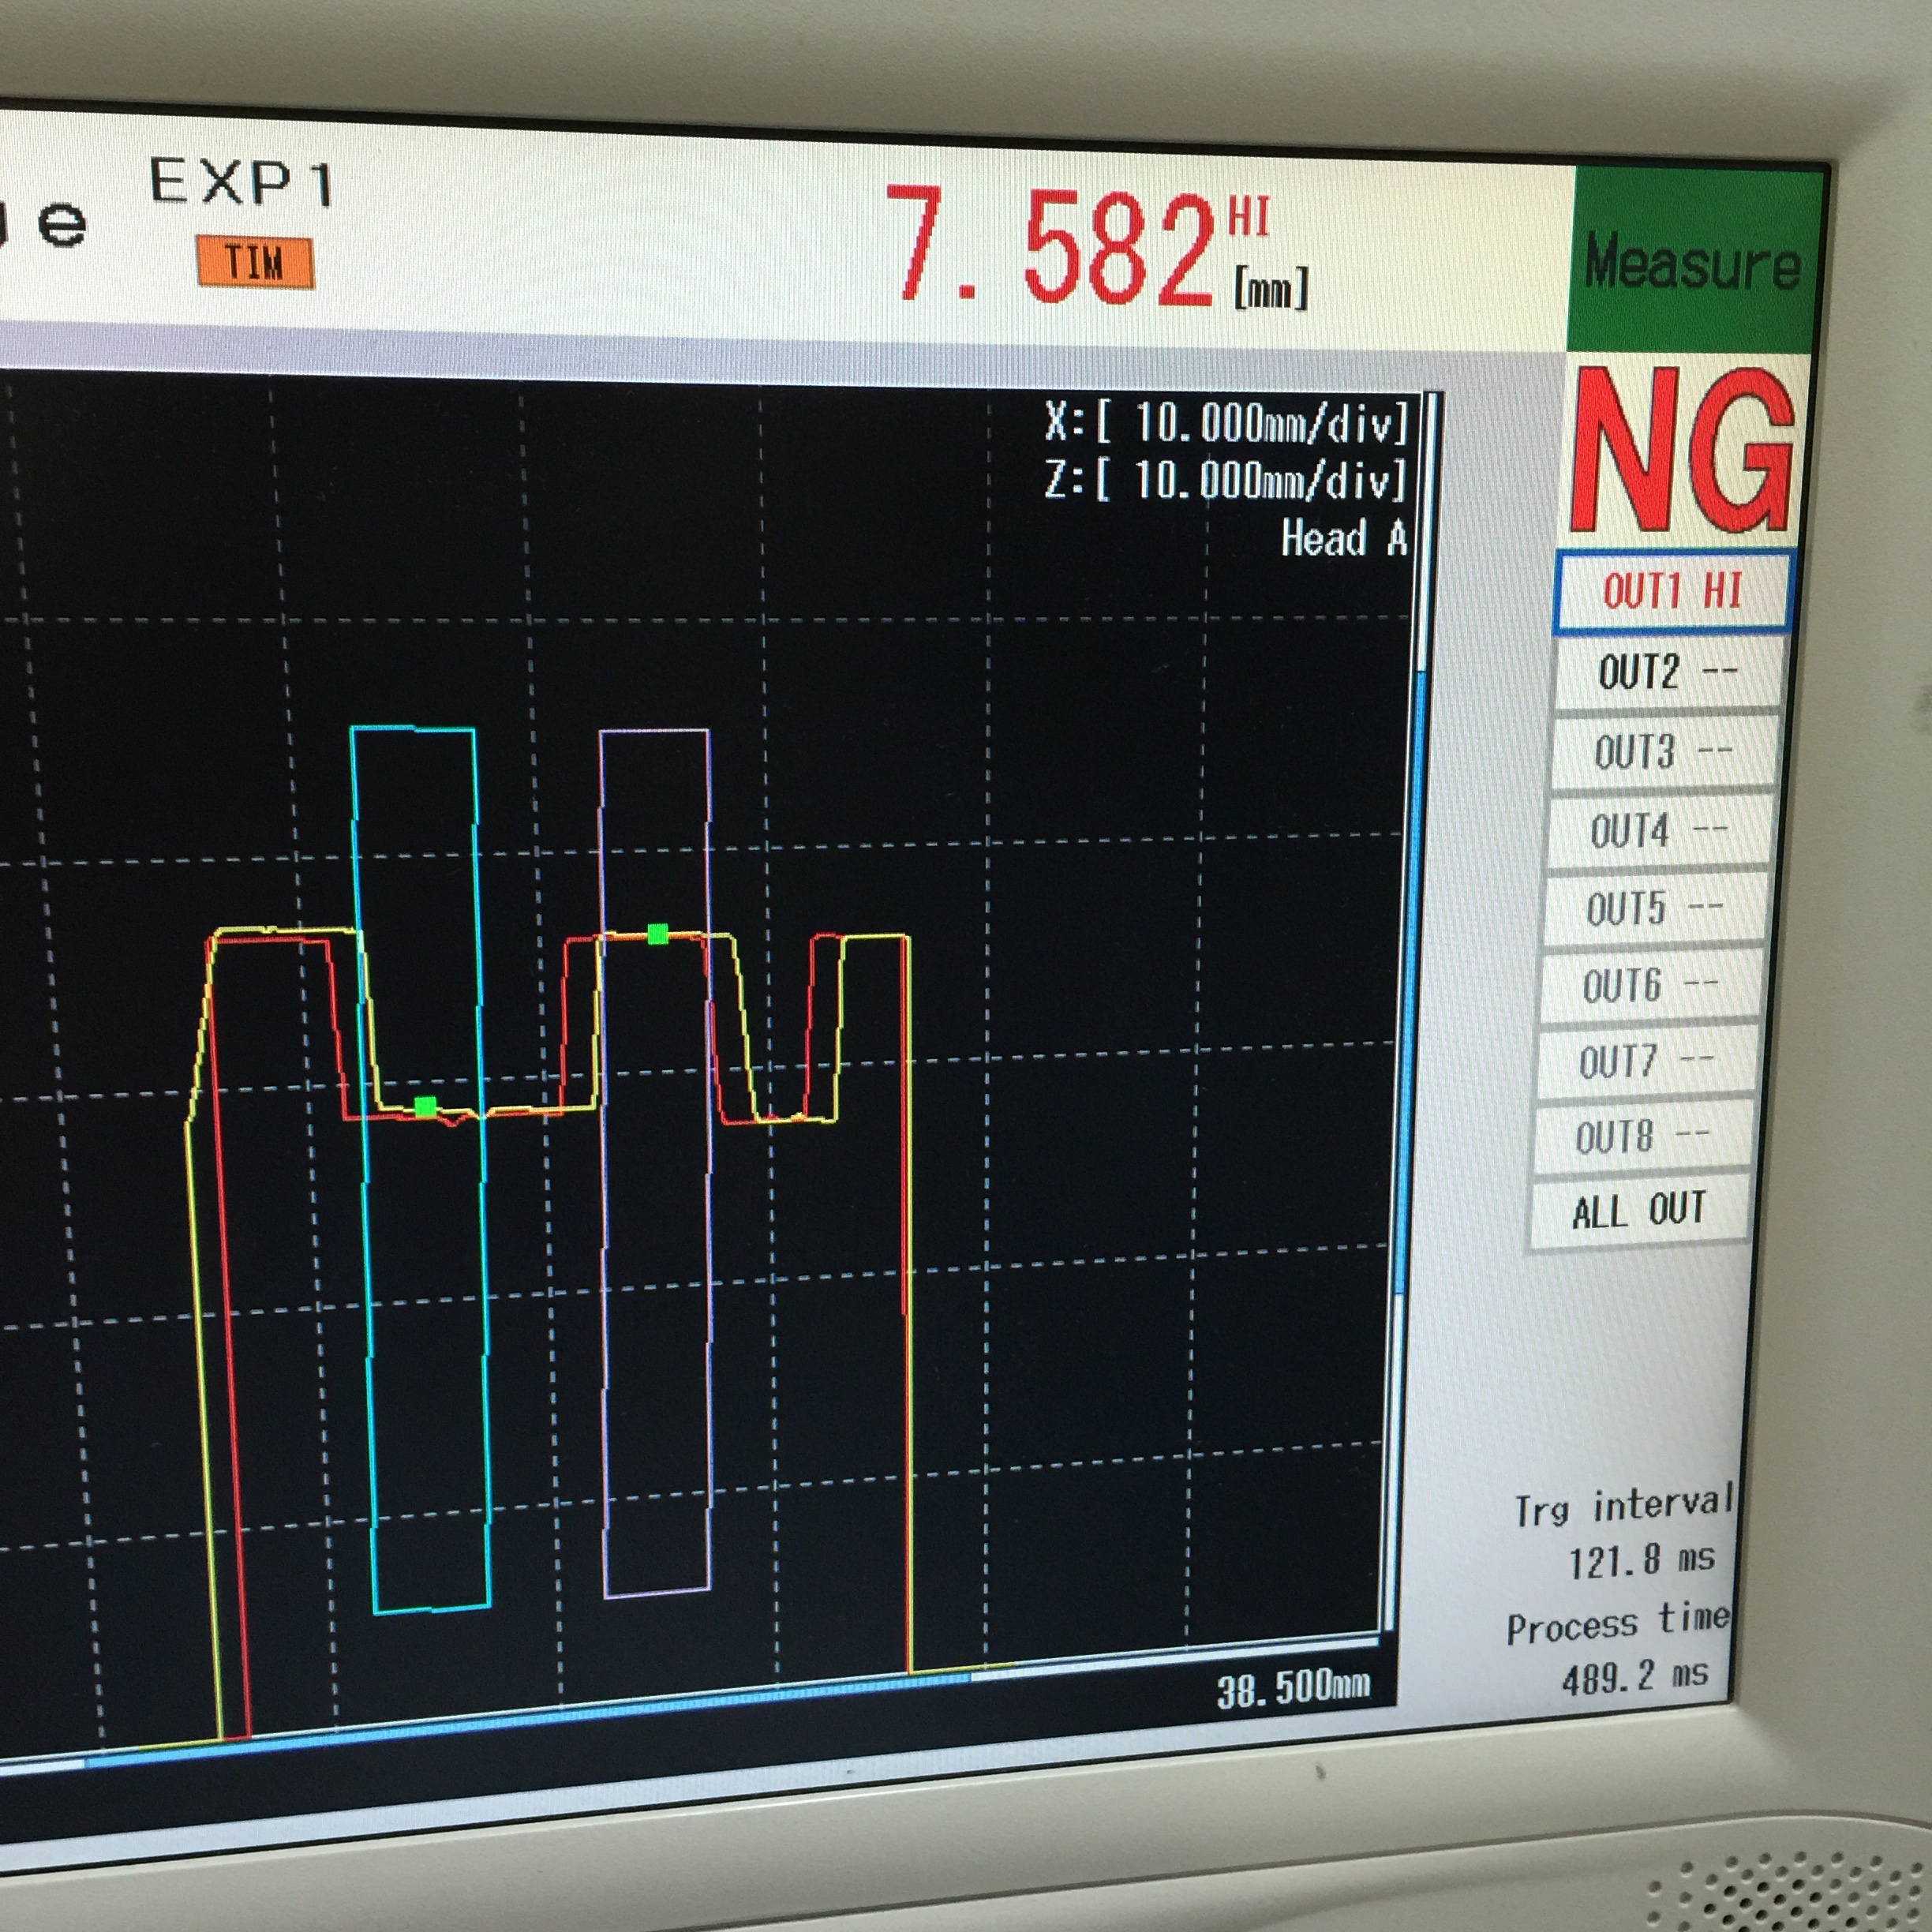
\includegraphics[width=0.4\linewidth]{Lab6/Step4.JPG}
	}
	\caption{Position correlation for Step measurement}
	\label{fig:two}
\end{figure}

\section*{Angle Measurement on Shiny Surface}
In this part, we try to measure the angle of an object with shiny surface and several small holes, shown in Figure \ref {fig:three}. \\ 

\begin{figure}[H]
	\centering
	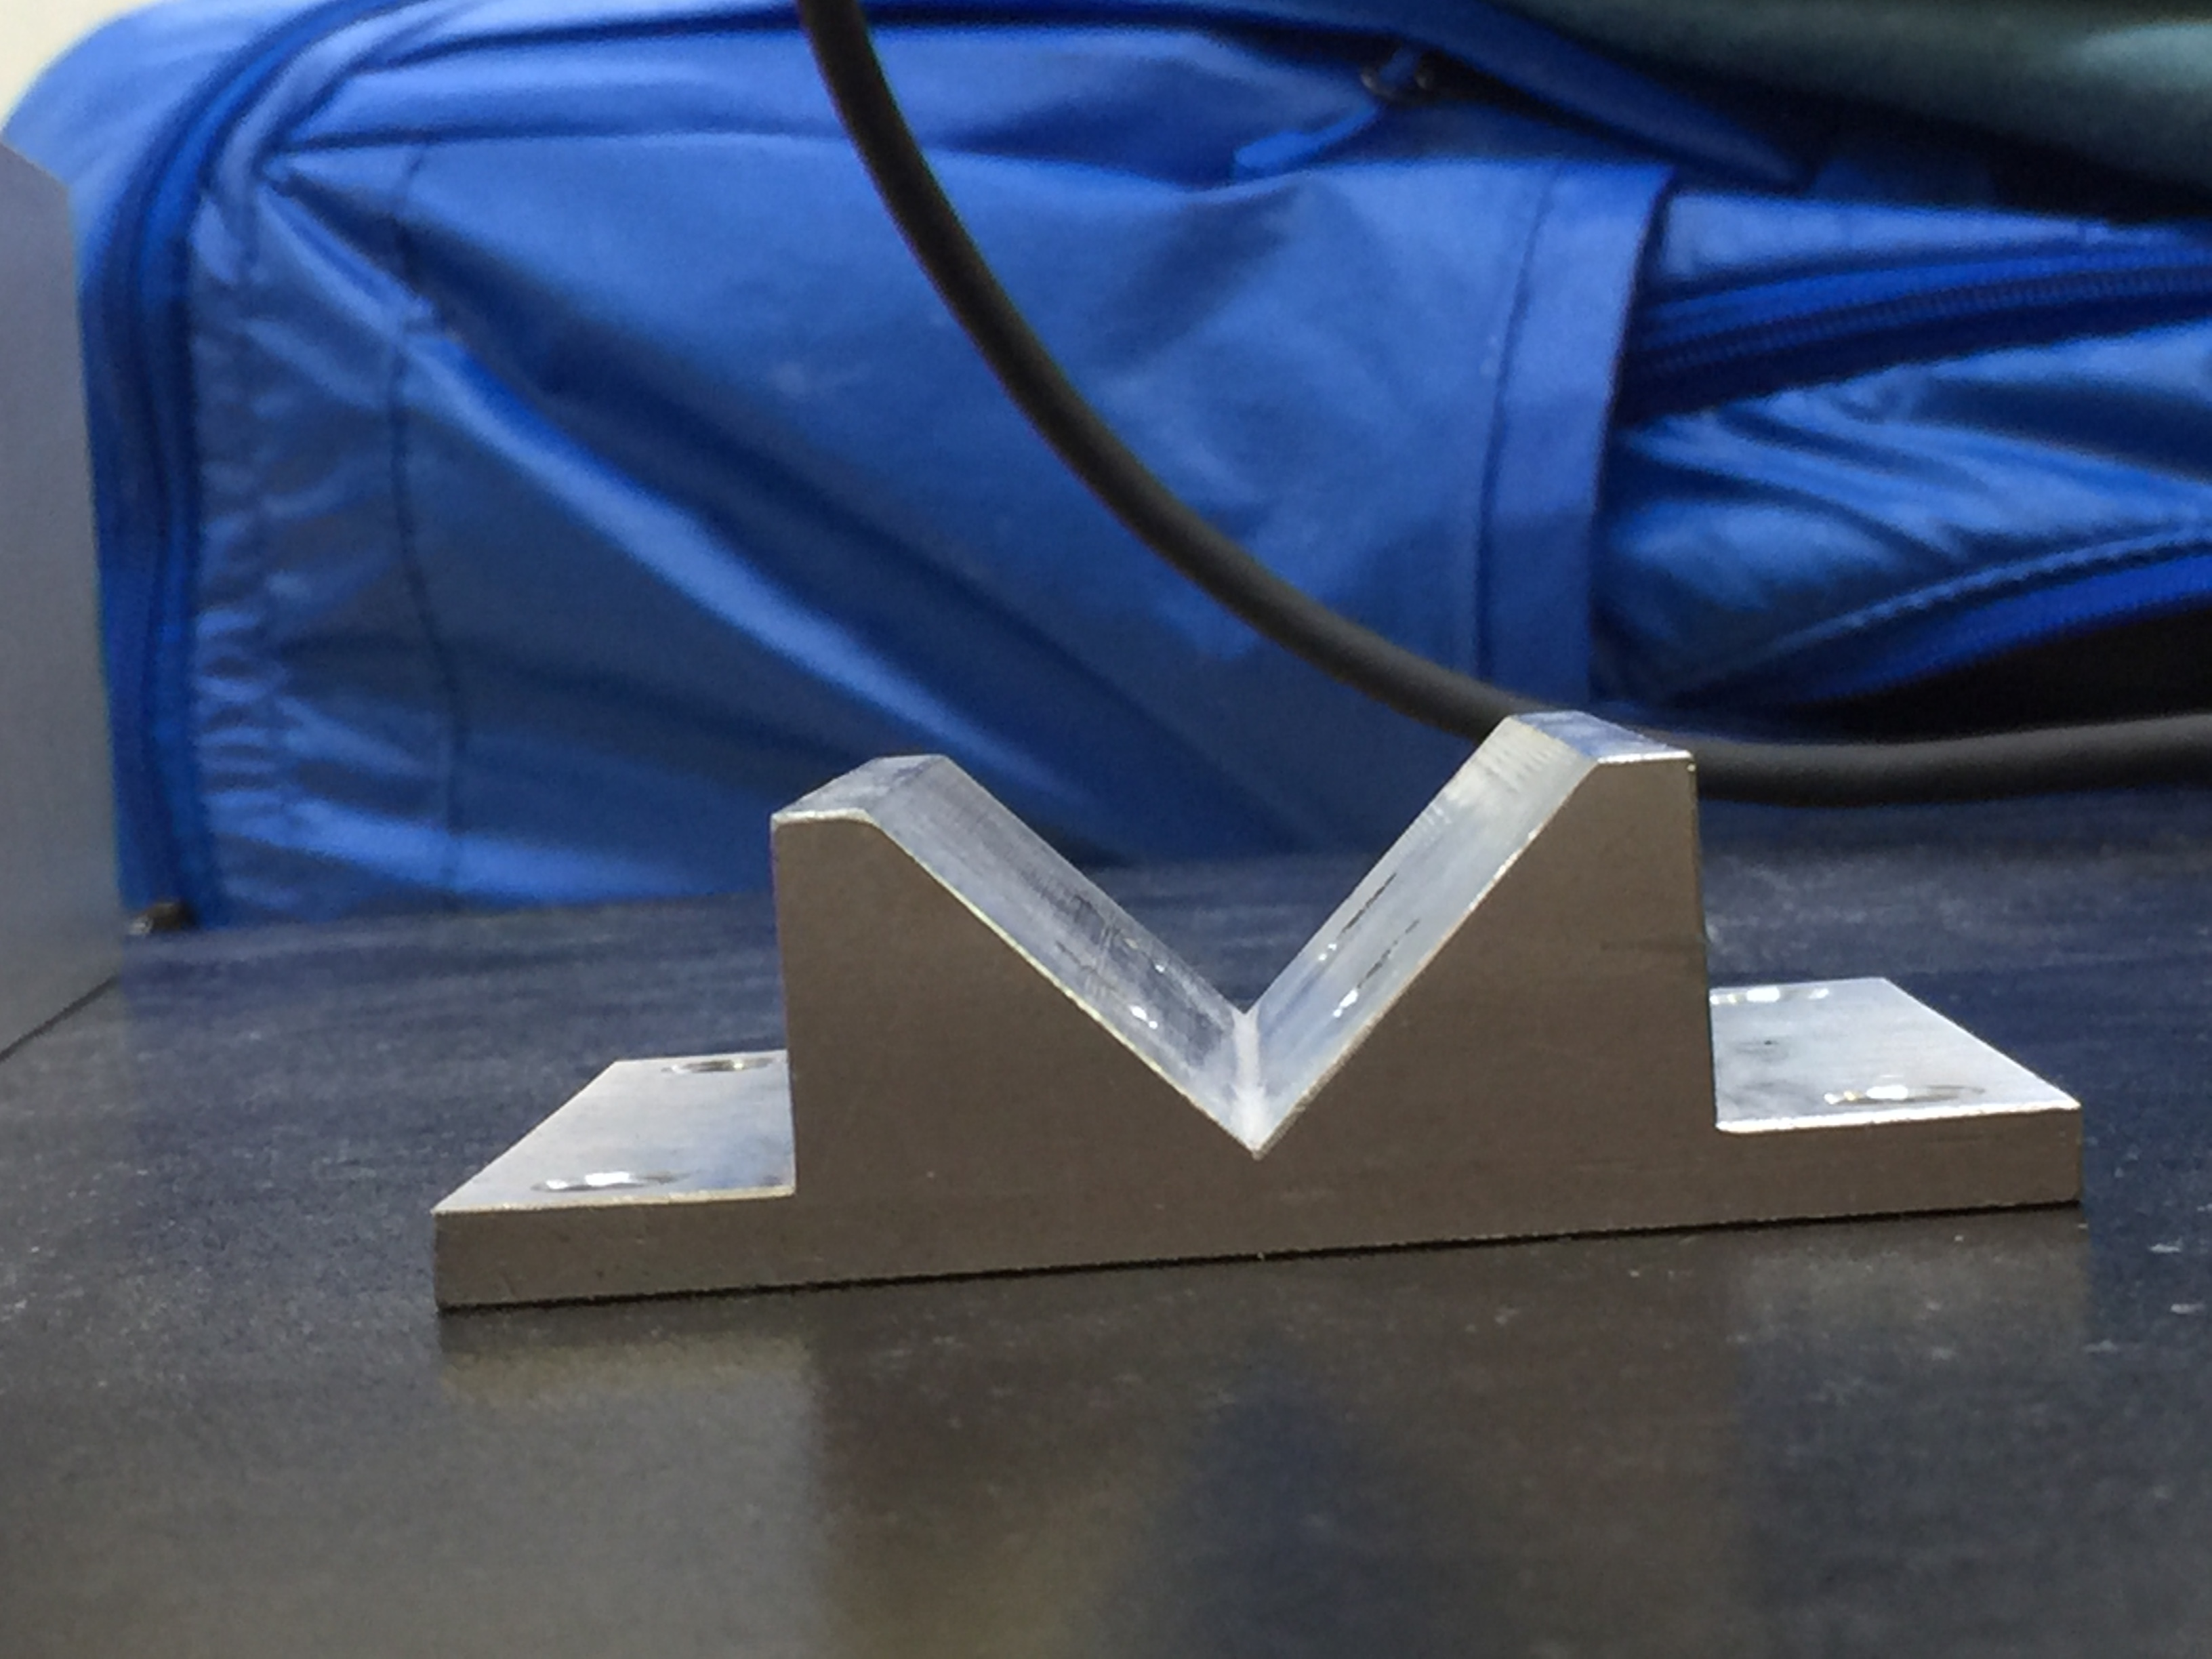
\includegraphics[width=0.8\linewidth]{Lab6/Angle5.JPG}
	\caption{Object with shiny surface}
	\label{fig:three}
\end{figure}

In order to characterize the angle between two planes, similarly, we should first adjust camera to a proper height so that we can get a good profile of the object. Then use "Master reg" to save the profile. Finally, the measurement type in "OUT setting" should be set to "Angle" and the regions of interest are also adjusted to a proper position, illustrated in Figure \ref{fig:four}. And the angle can be easily measured from the regions of interest.\\

\begin{figure}[H]
	\centering
	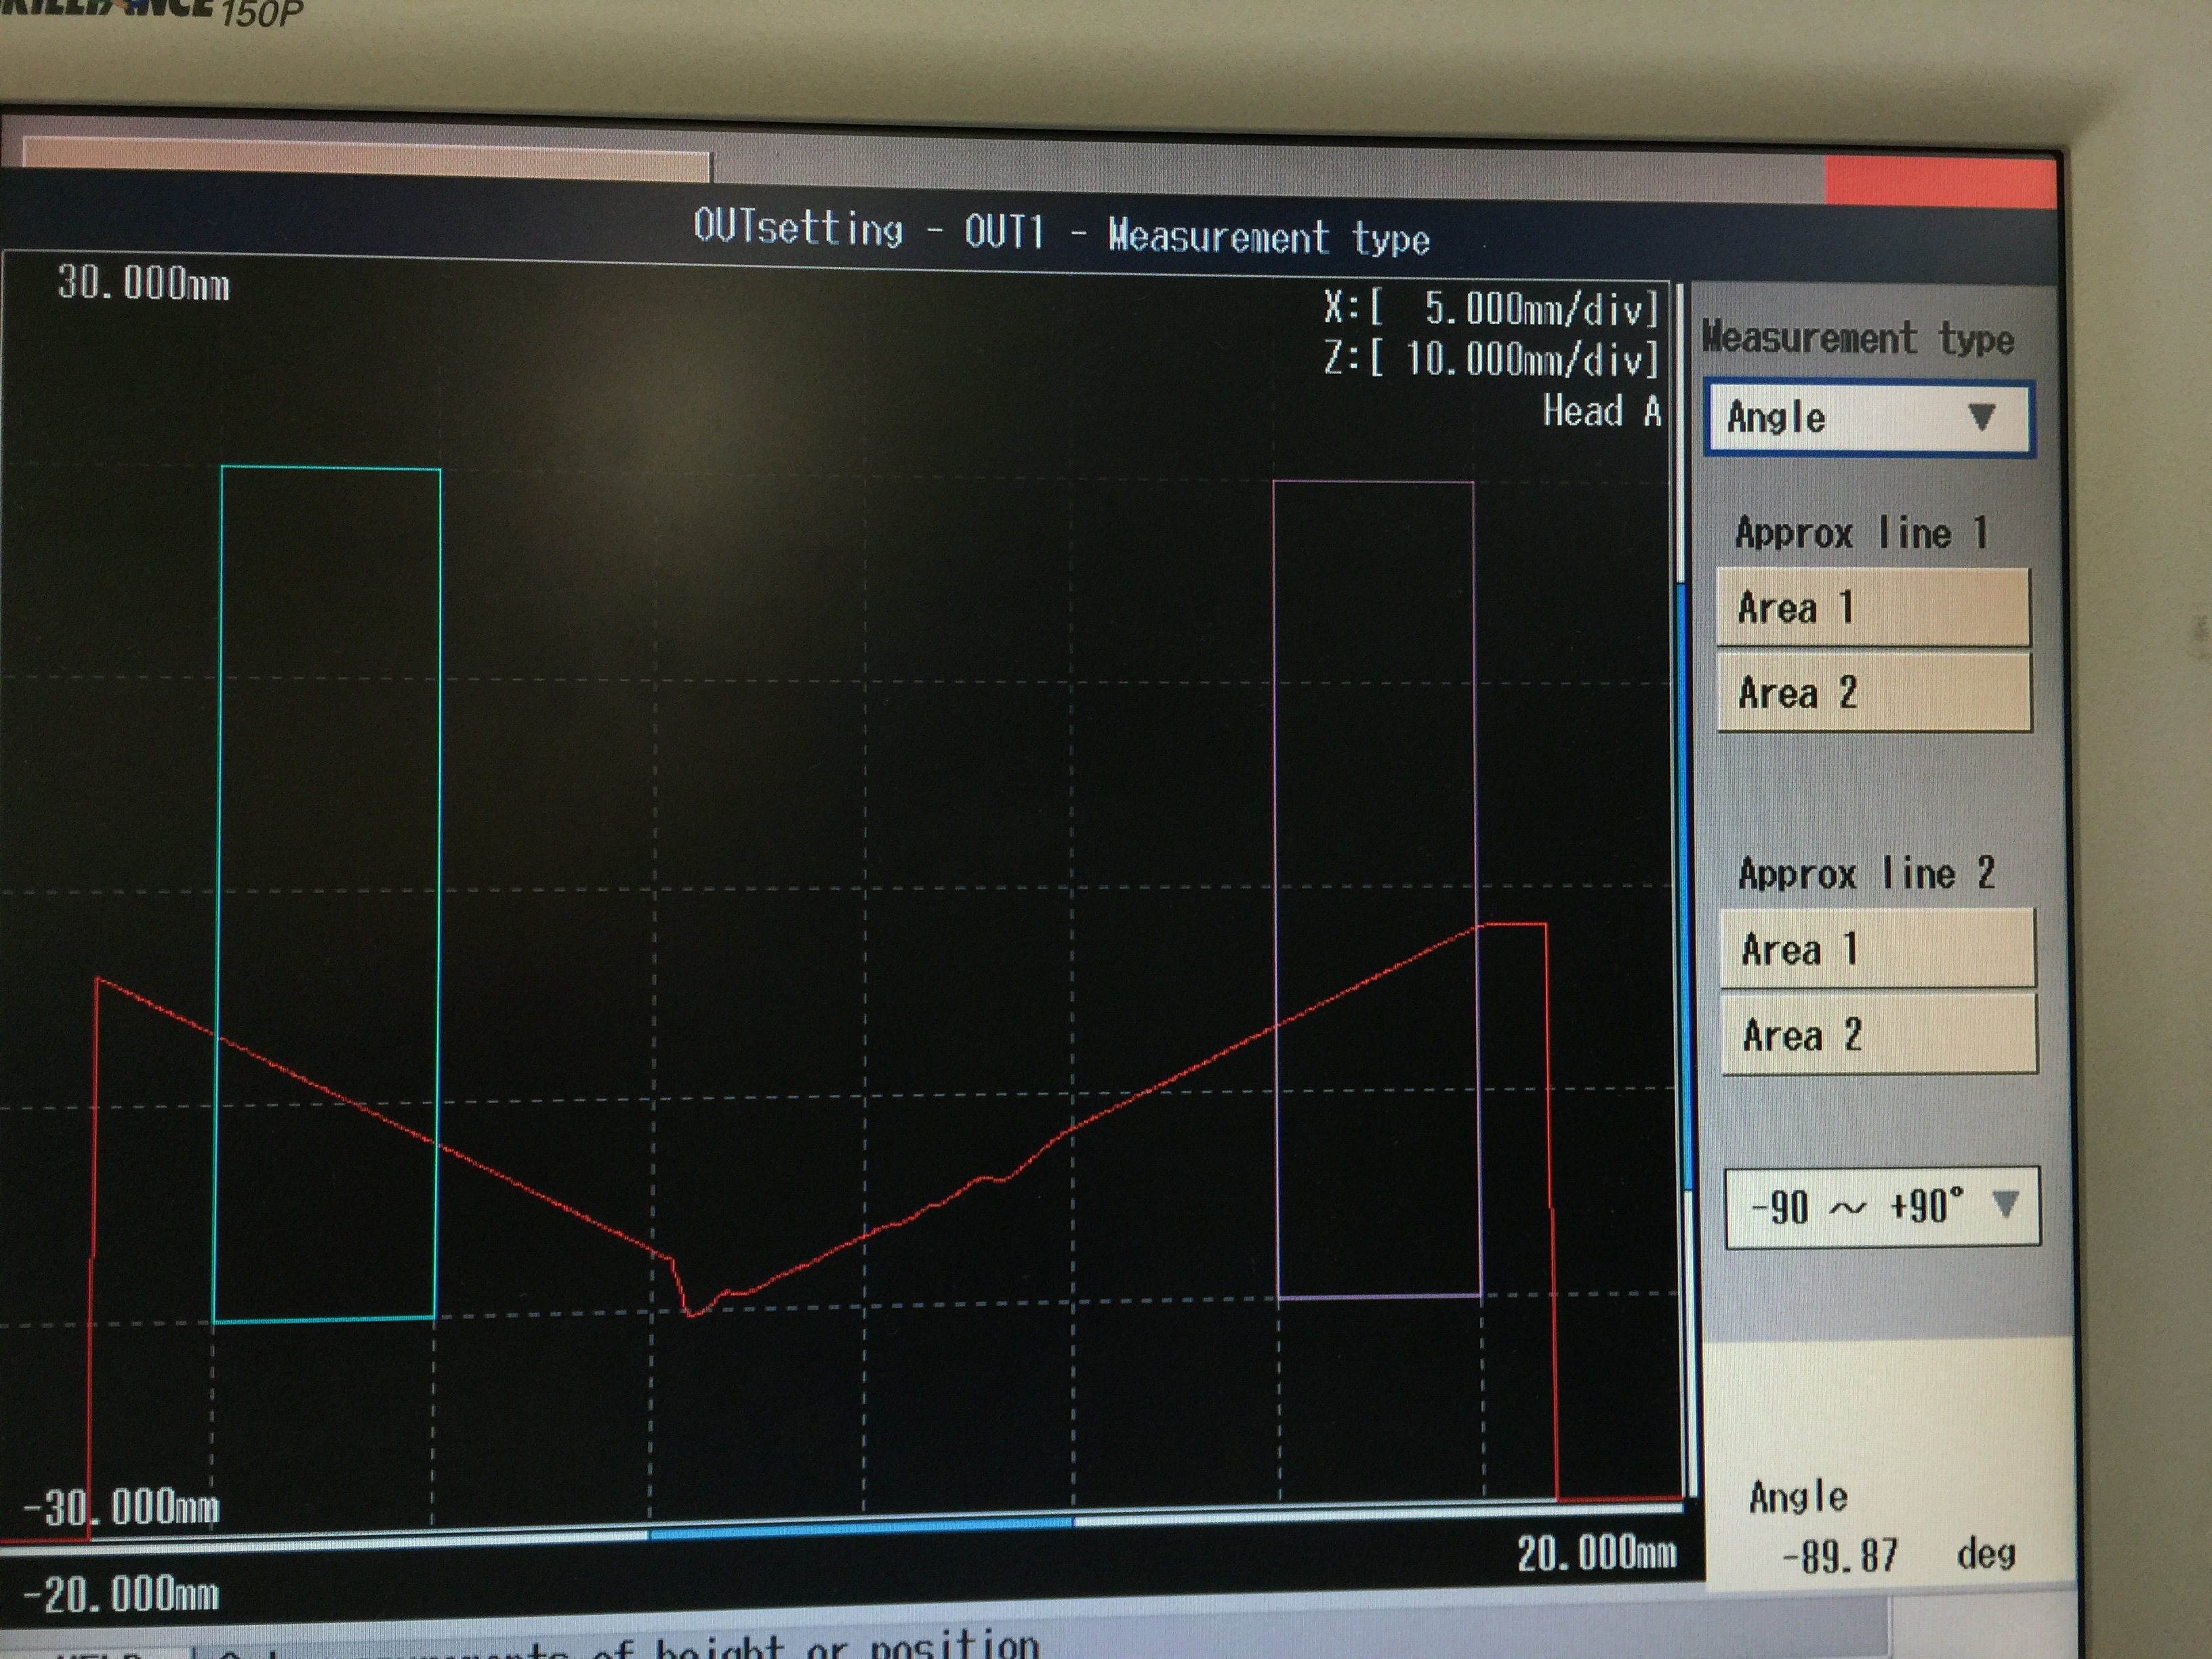
\includegraphics[width=0.8\linewidth]{Lab6/Angle1.JPG}
	\caption{Profile and regions of interest of object}
	\label{fig:four}
\end{figure}

Naturally, we want to improve the measurement by position adjustment. After doing the similar procedure to set position correction as in the previous part, we get the result. Figure \ref{fig:fivea} and Figure \ref{fig:fiveb} are two measurements when the object is shifted or rotated in two different way. We find that both outcomes can give us really good measurements, despite the movement of the object. 

\begin{figure}[H]
	\centering
	\subfigure[Original]{\label{fig:fivea}
	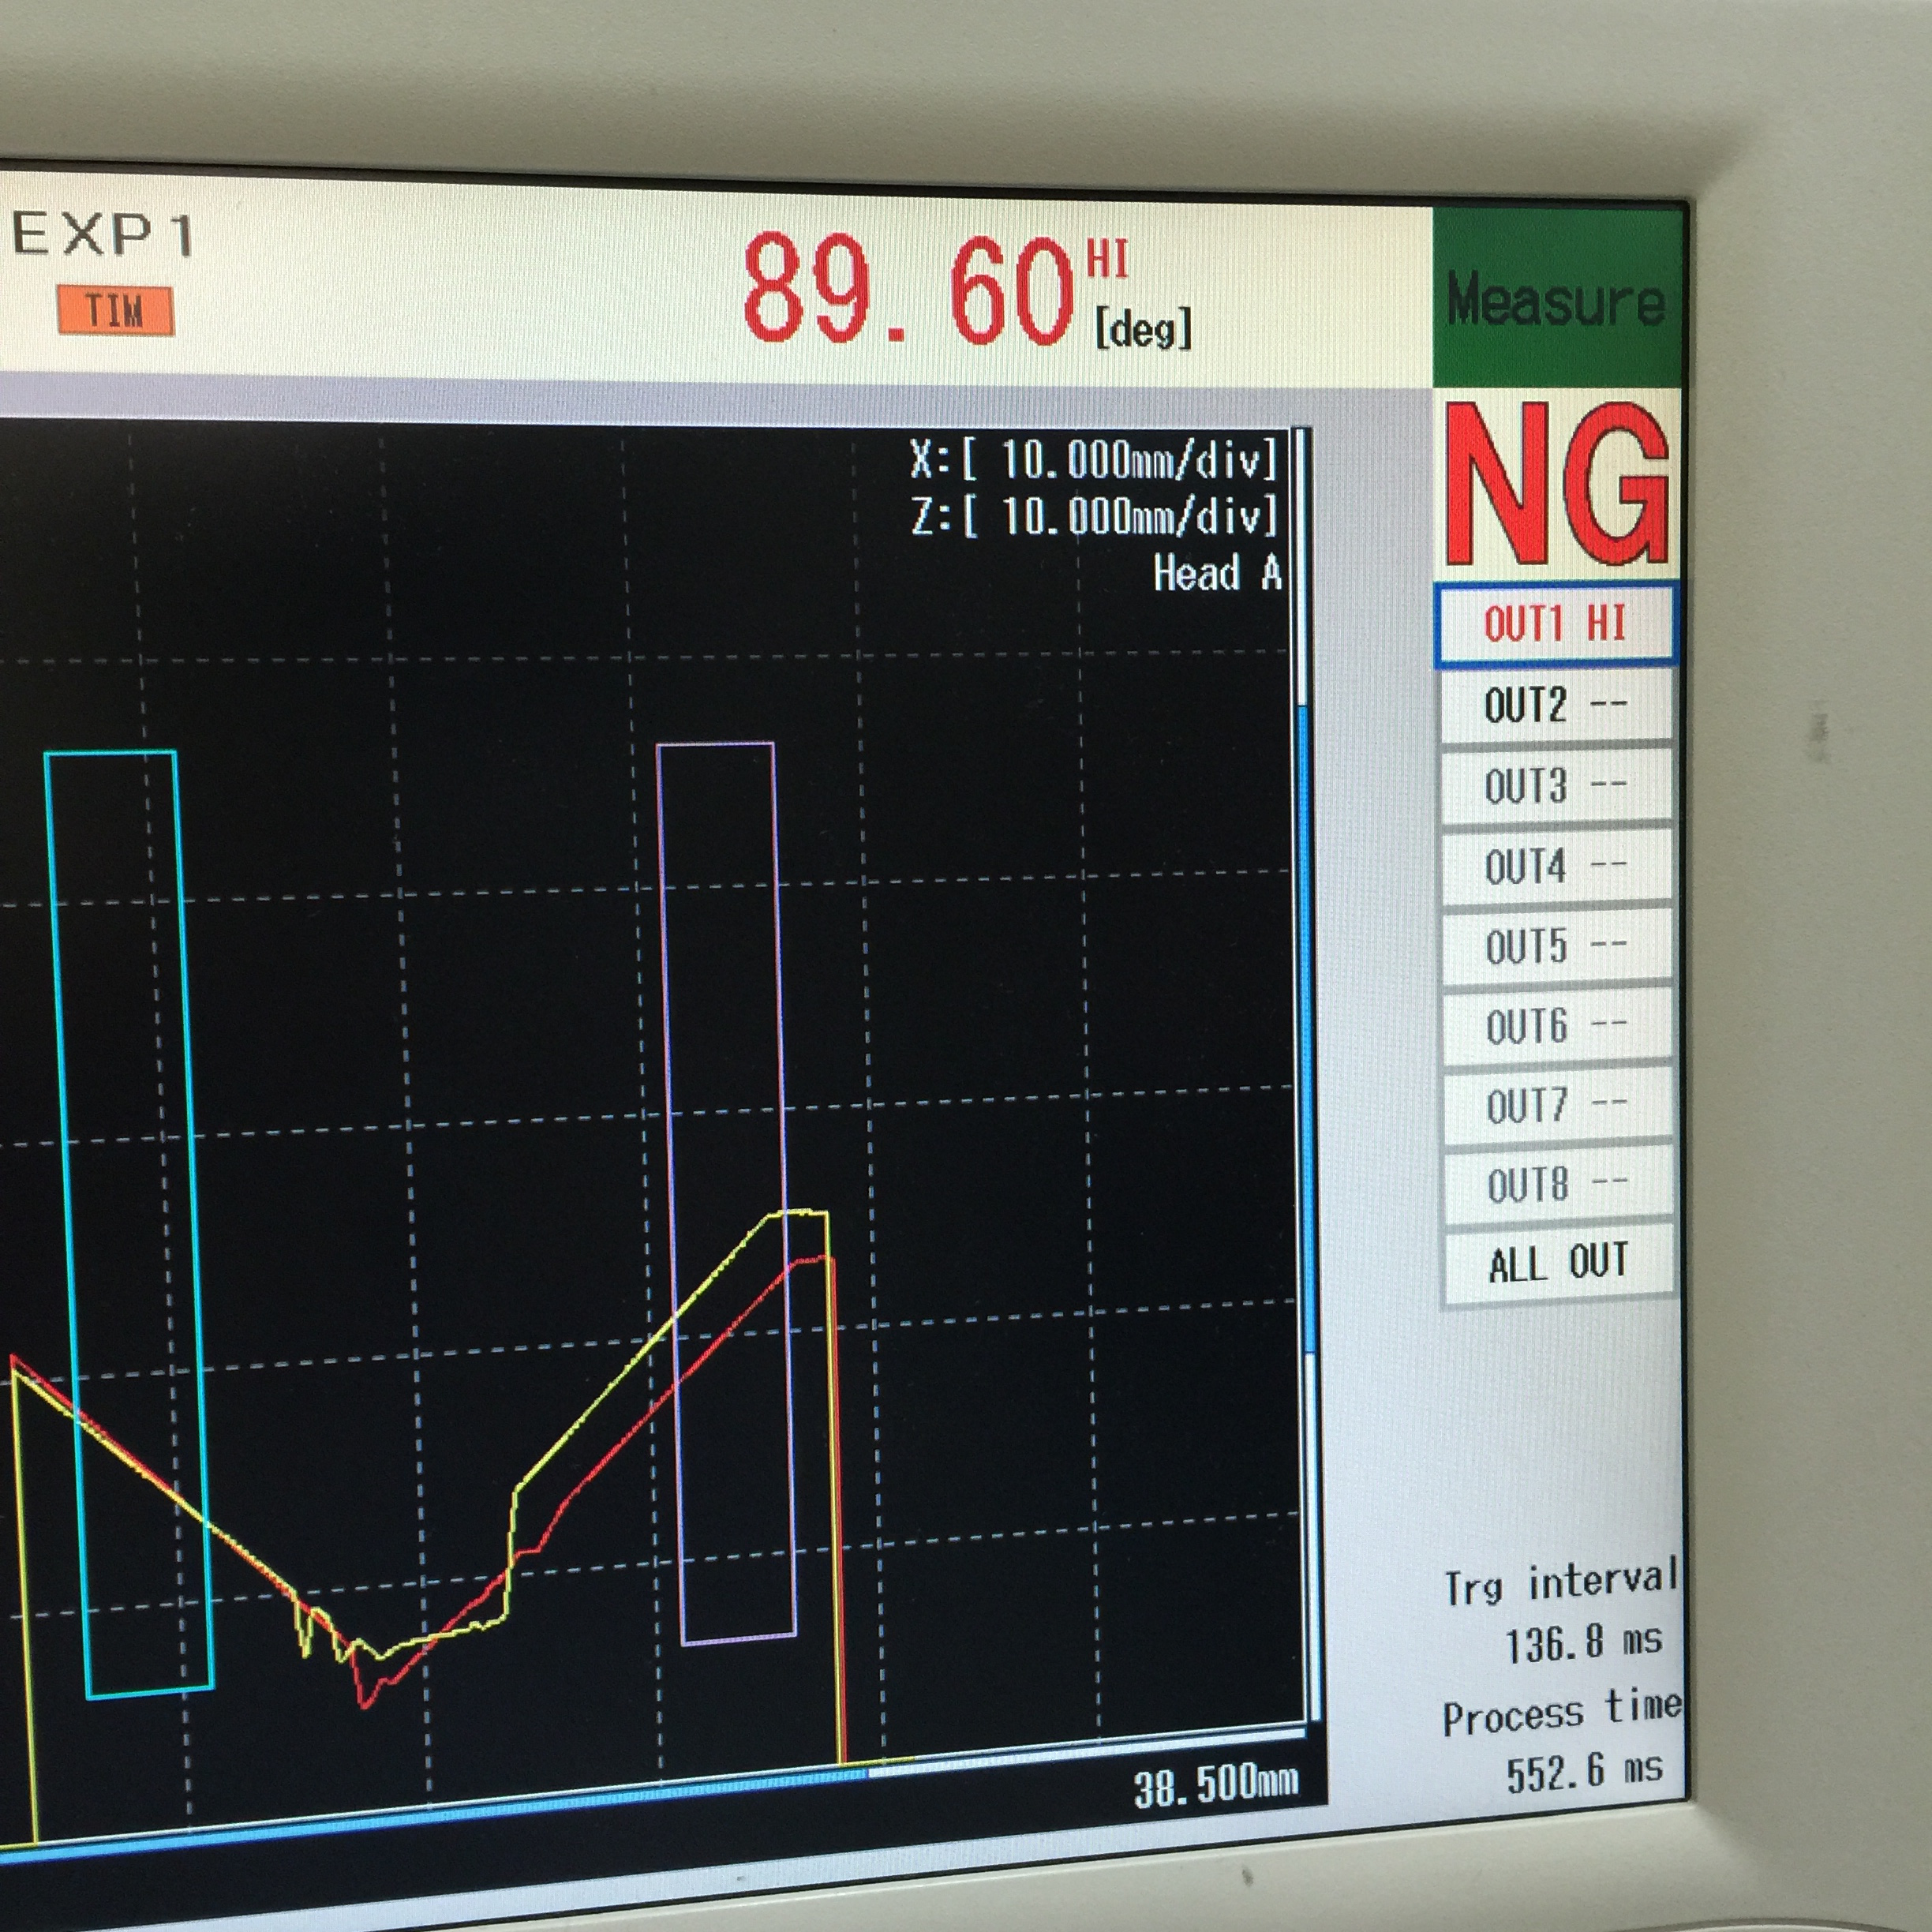
\includegraphics[width=0.4\linewidth]{Lab6/Angle3.JPG}
	}
	\subfigure[Shift and Angle]{\label{fig:fiveb}
	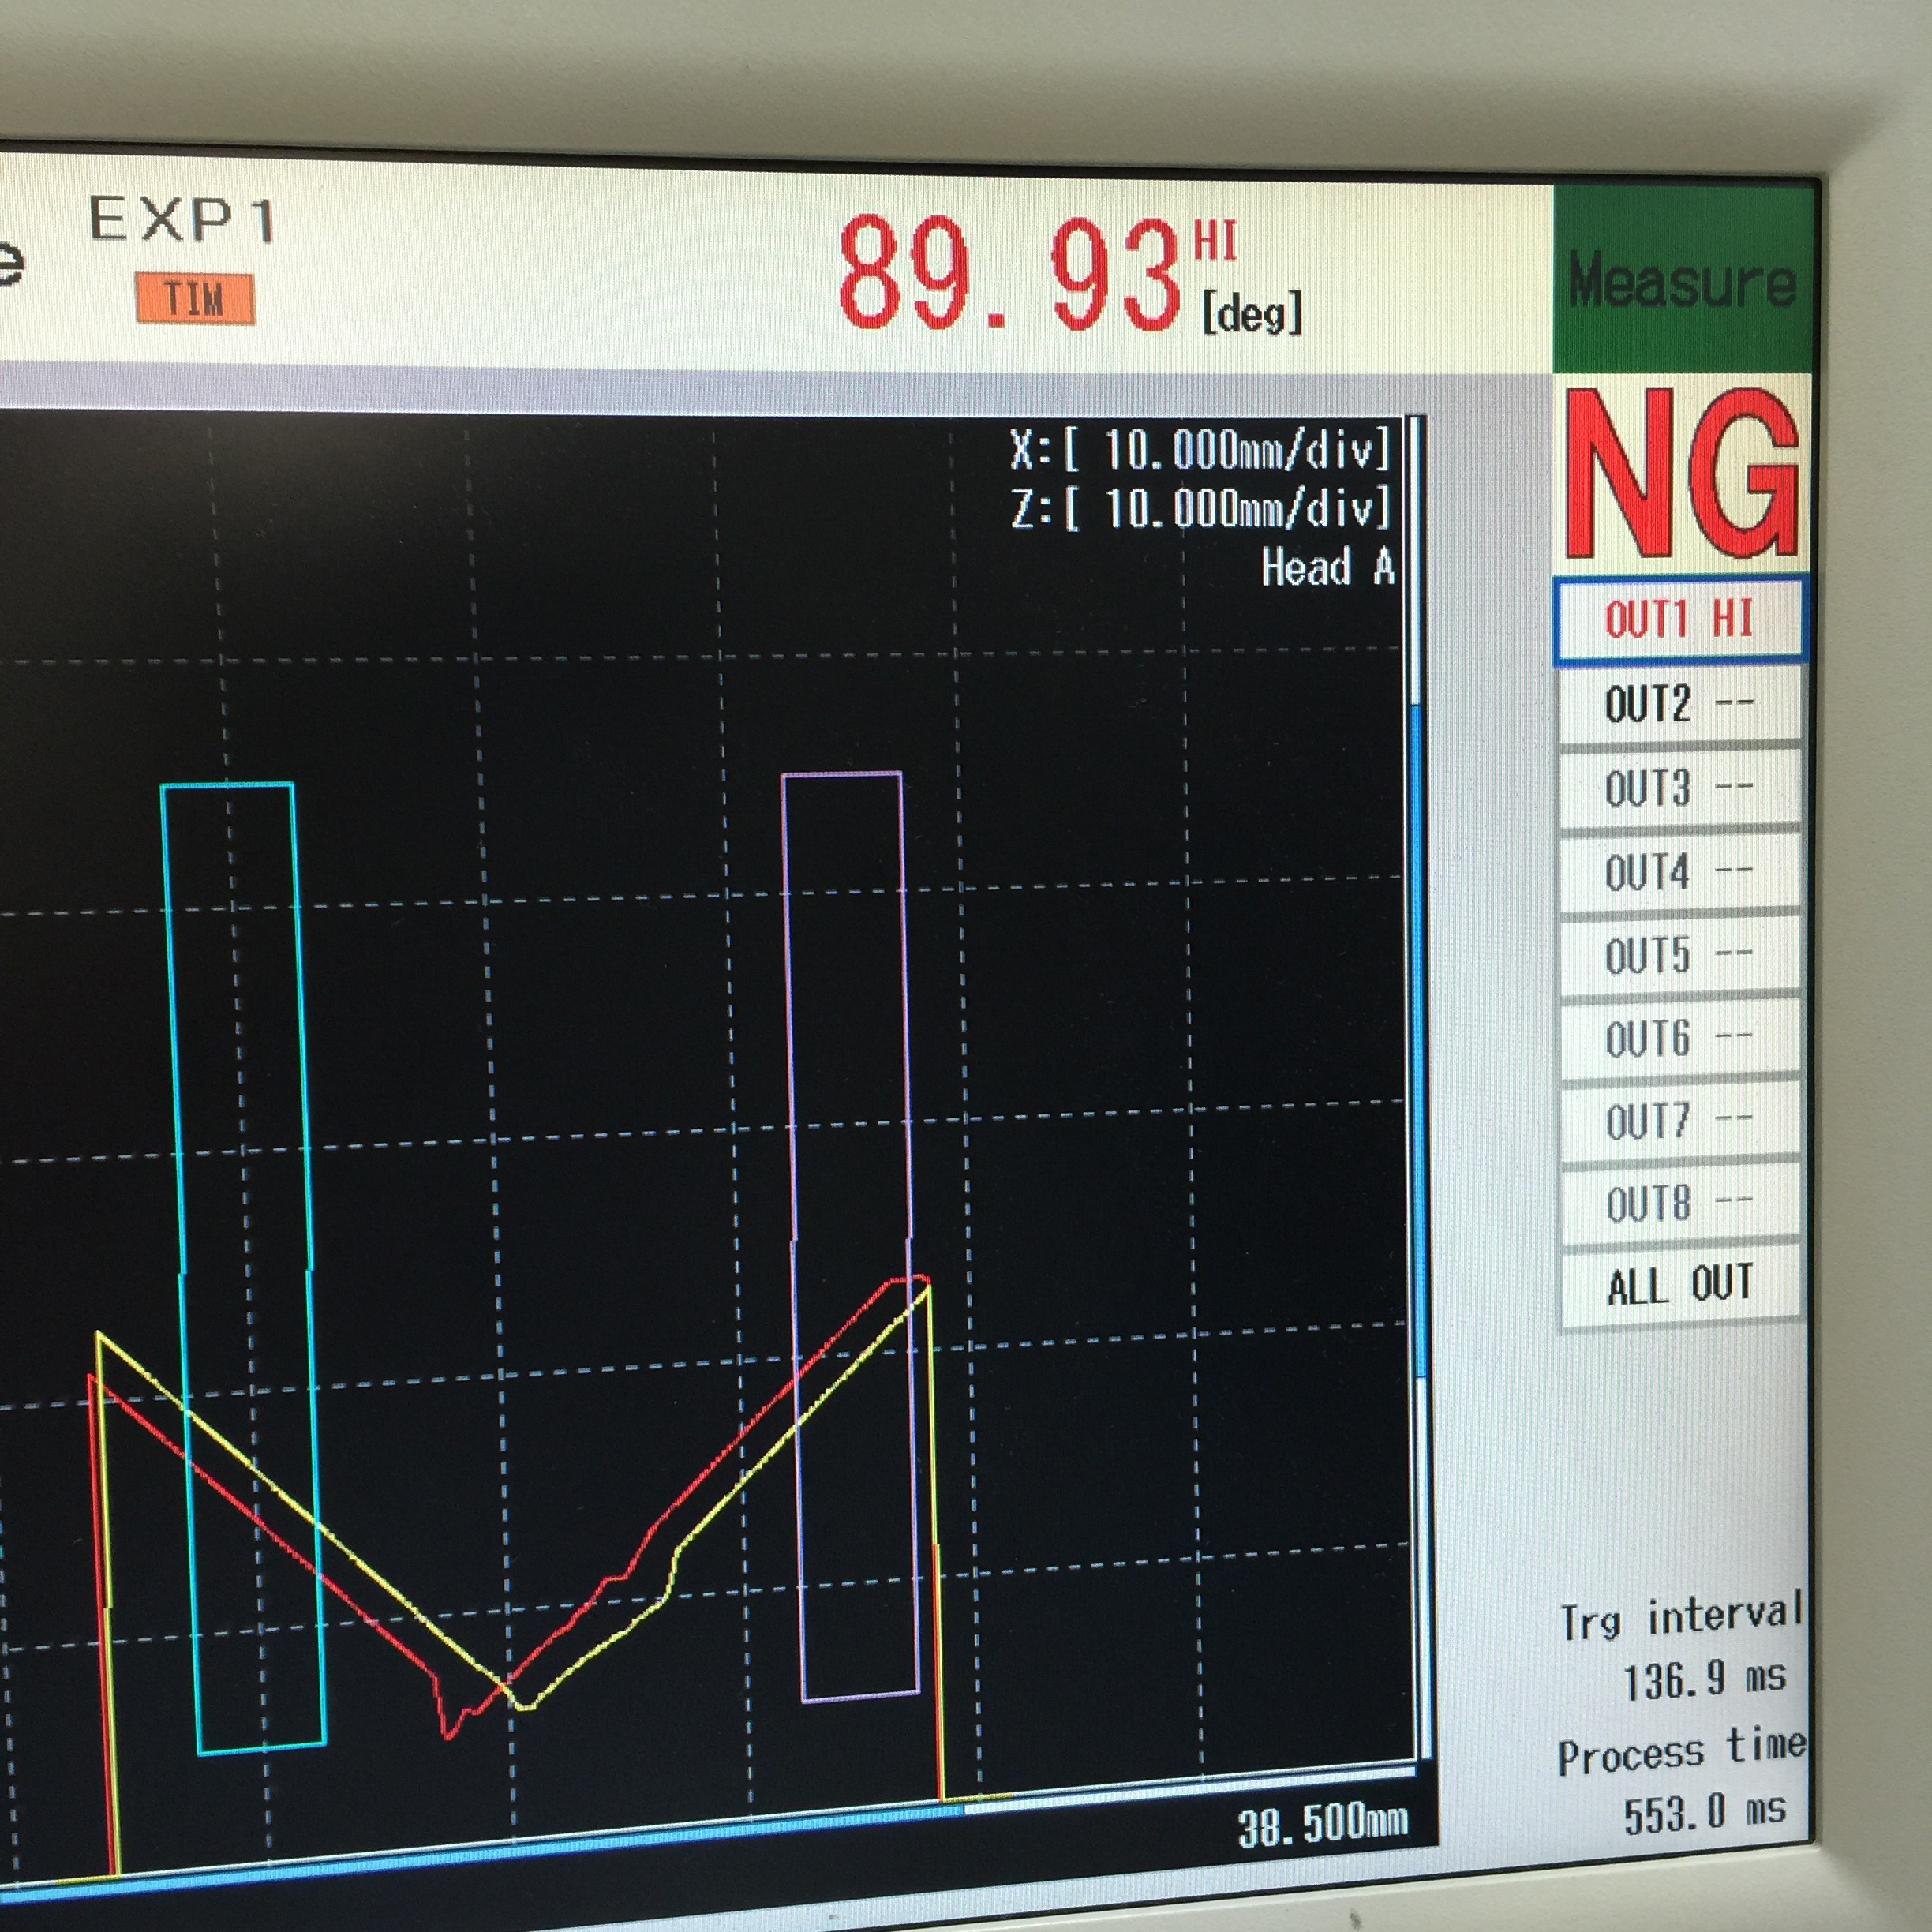
\includegraphics[width=0.4\linewidth]{Lab6/Angle4.JPG}
	}
	\caption{Measurement in different case of shift and rotation}
	\label{fig:five}
\end{figure}

Finally, in this part, we want to acquire the goal of hole detection. First, In Figure \ref{fig:sixa}, we can see there are different kinds of holes. And then, Figure \ref{fig:sixb} and Figure \ref{fig:sixc} reflect how the holes can be detected in the images during the measurement. 

\begin{figure}[H]
	\centering
	\subfigure[Holes in the object]{\label{fig:sixa}
	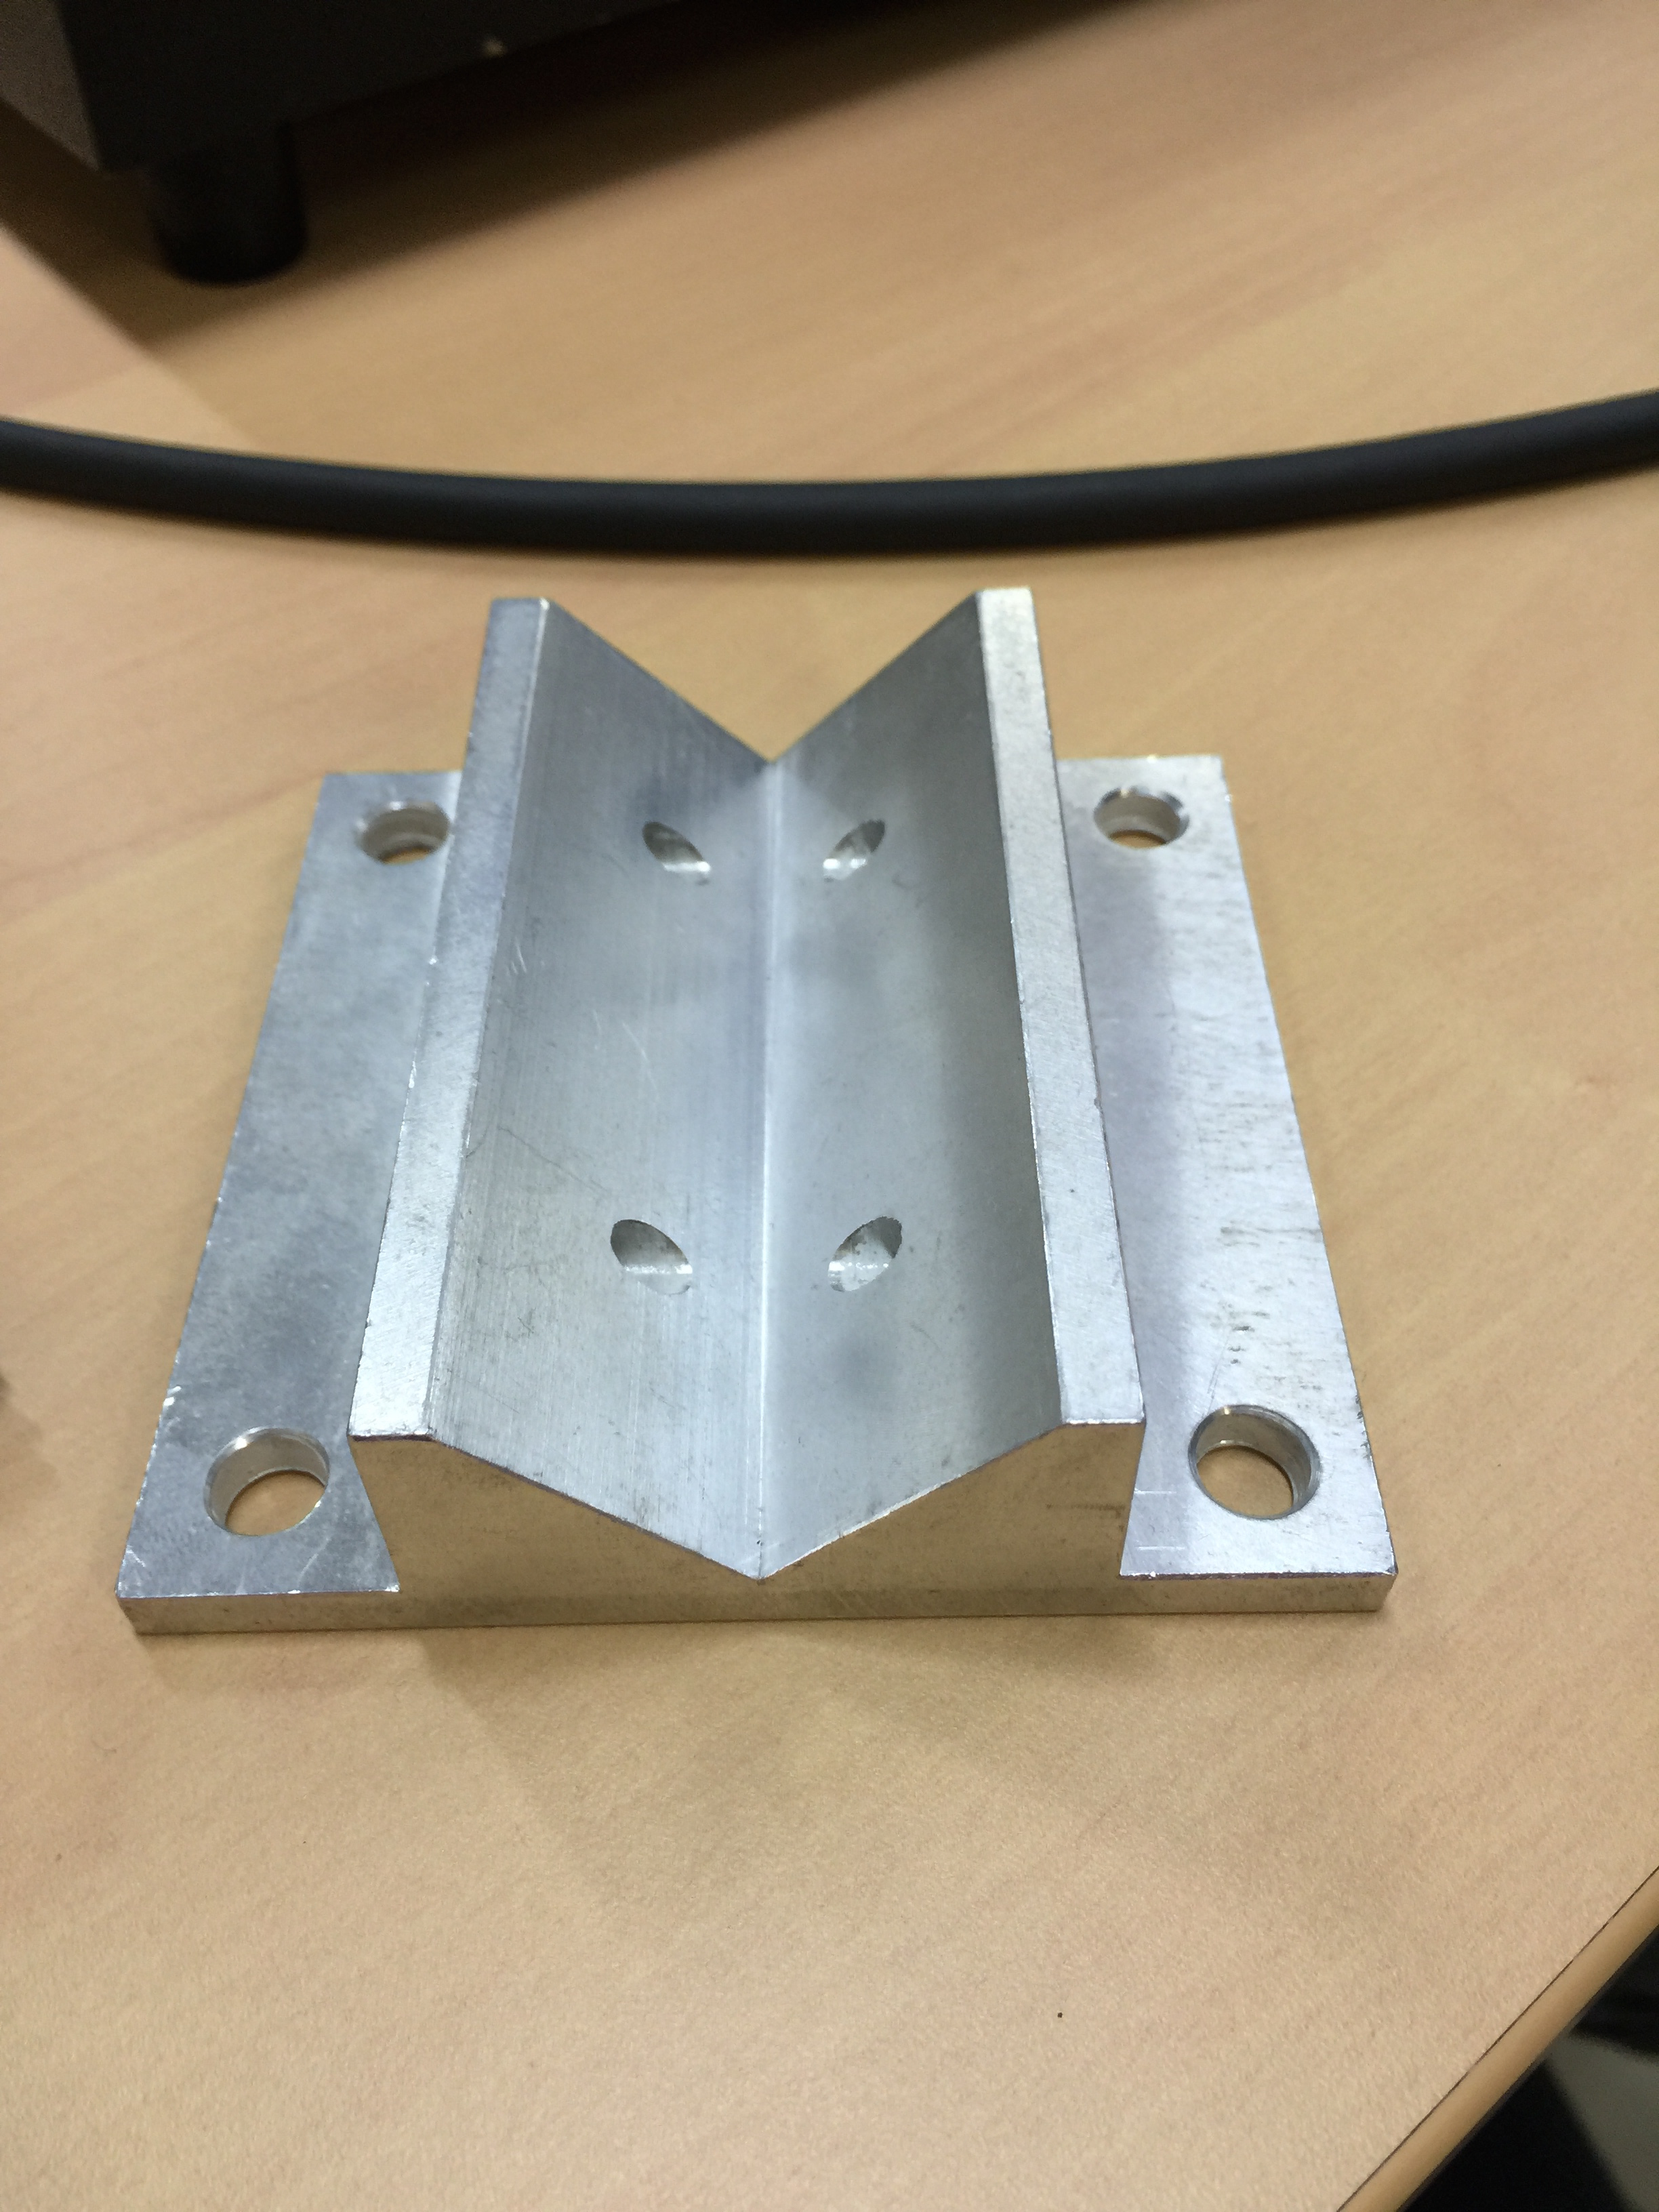
\includegraphics[width=0.6\linewidth]{Lab6/Hole3.JPG}
	}
	\subfigure[Hole in the side]{\label{fig:sixb}
	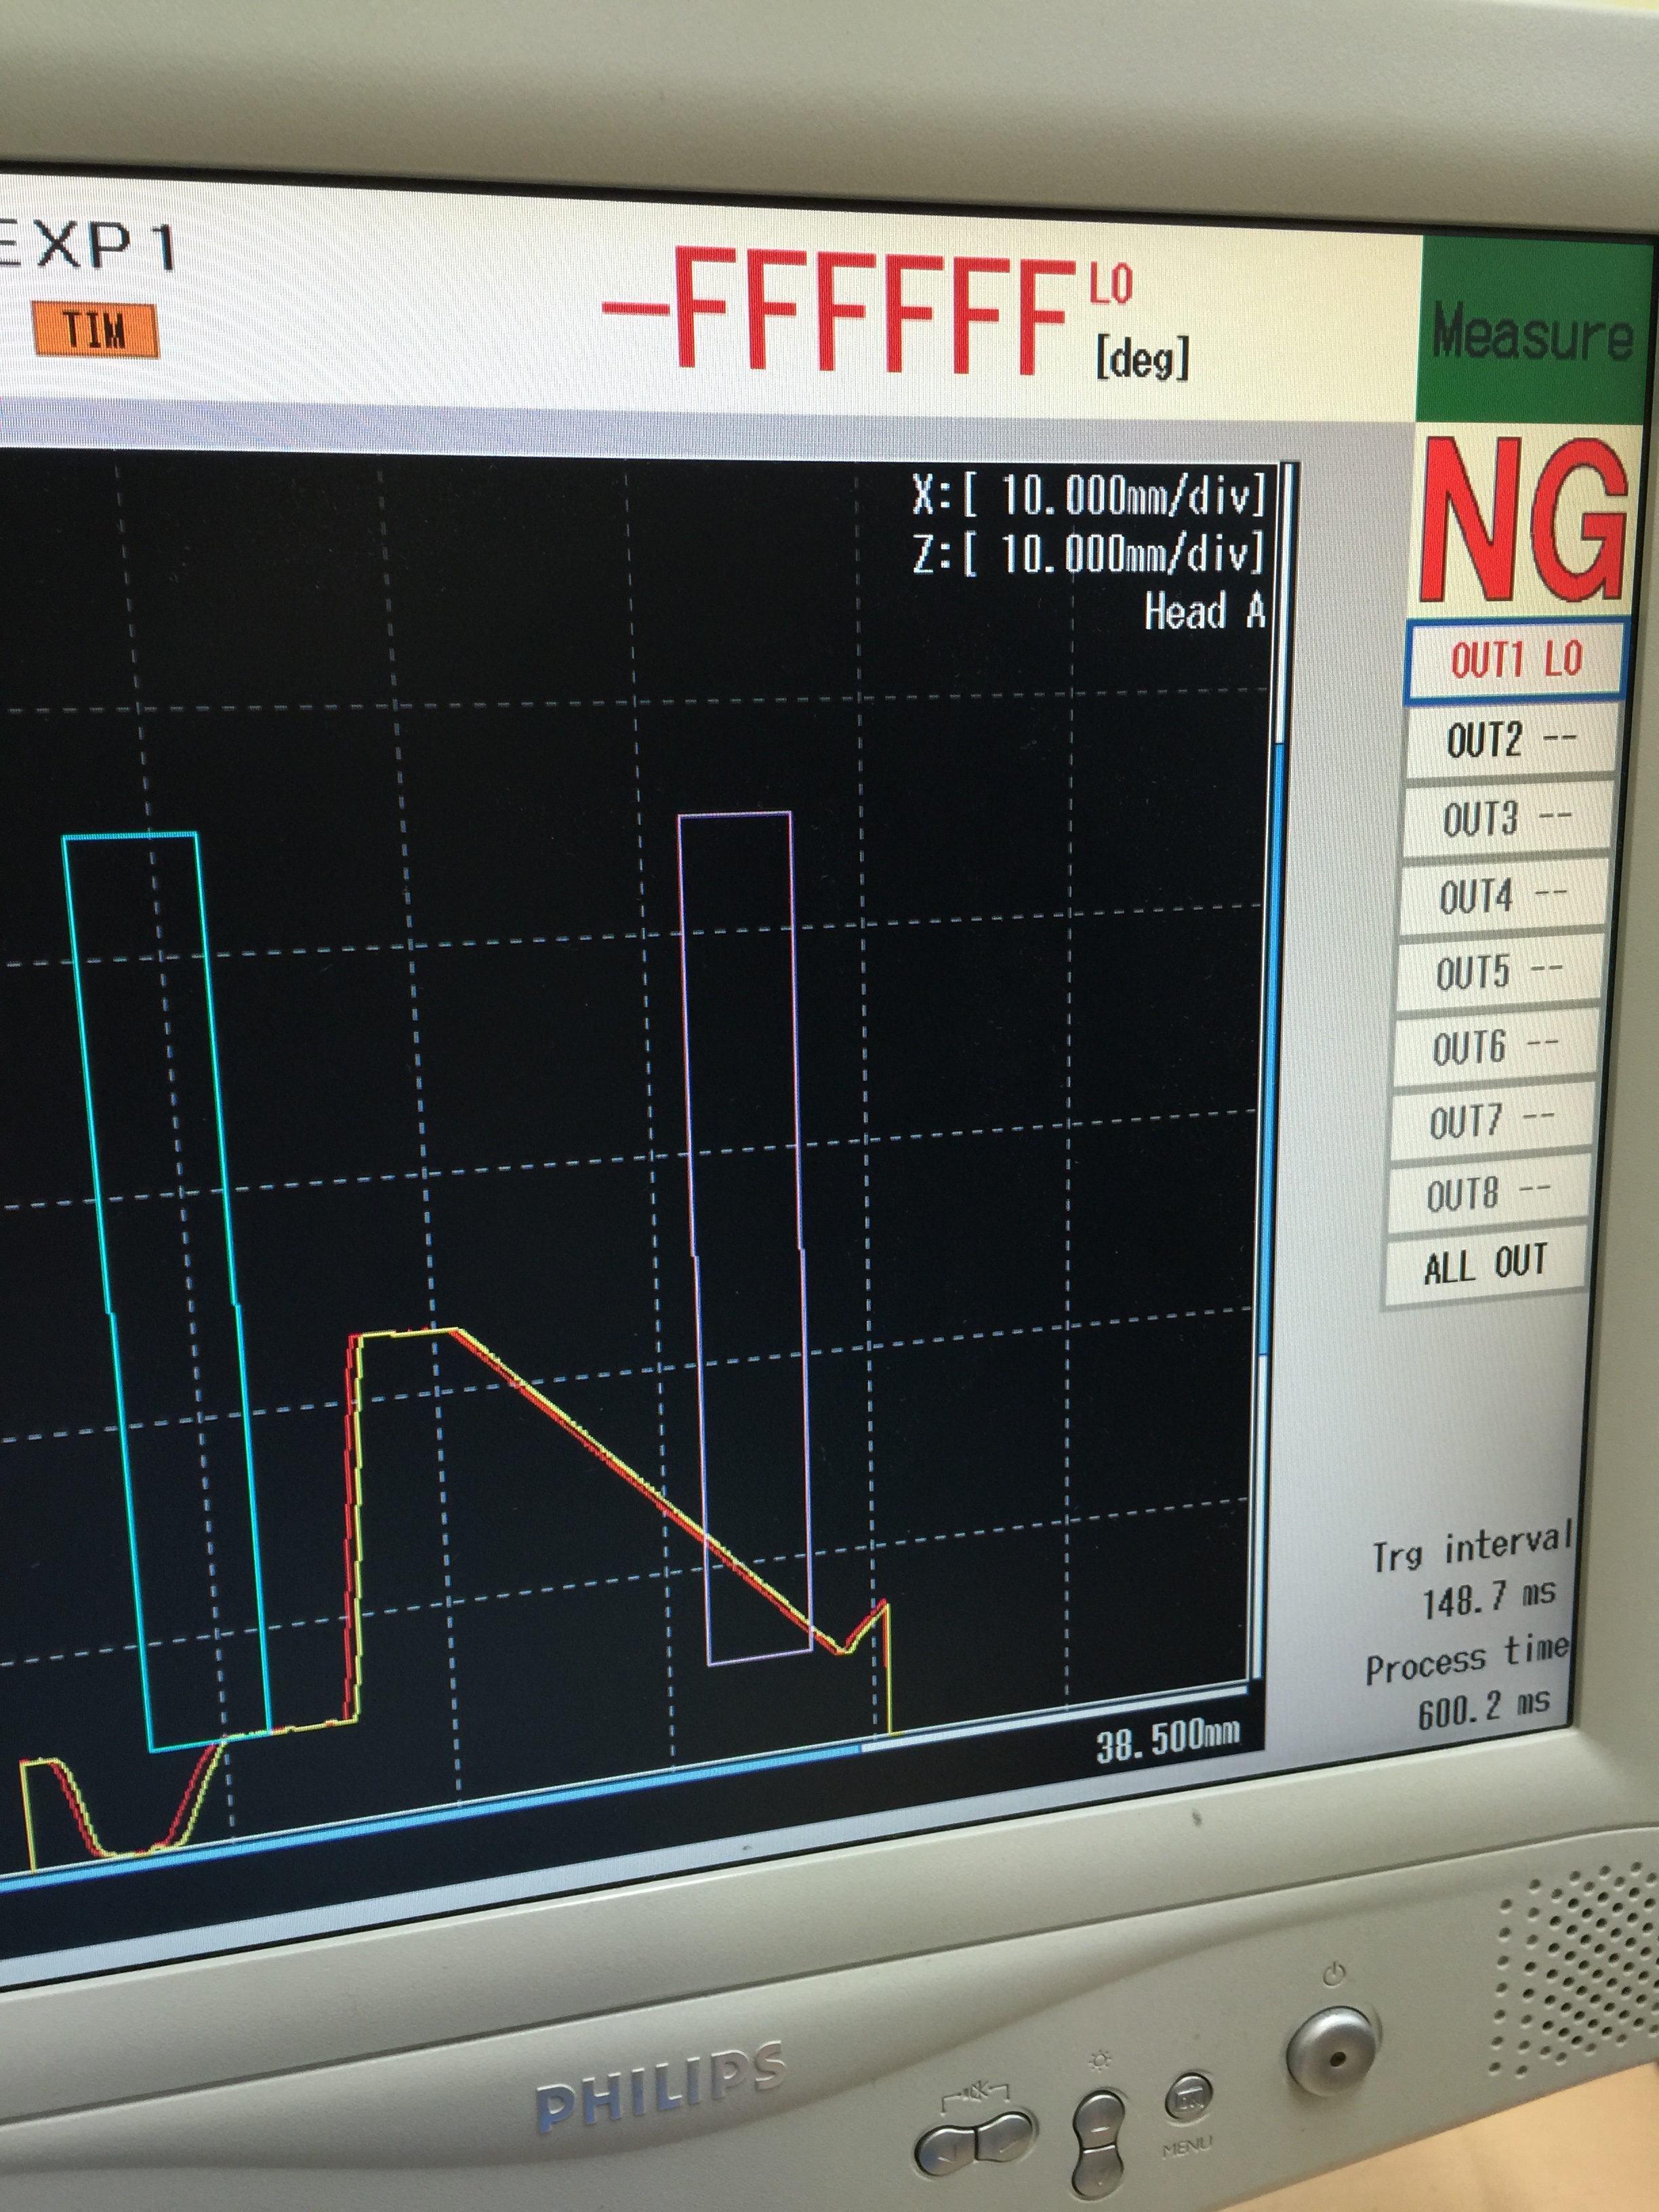
\includegraphics[width=0.45\linewidth]{Lab6/Hole1.JPG}
	}
	\subfigure[Hole in the planes]{\label{fig:sixc}
	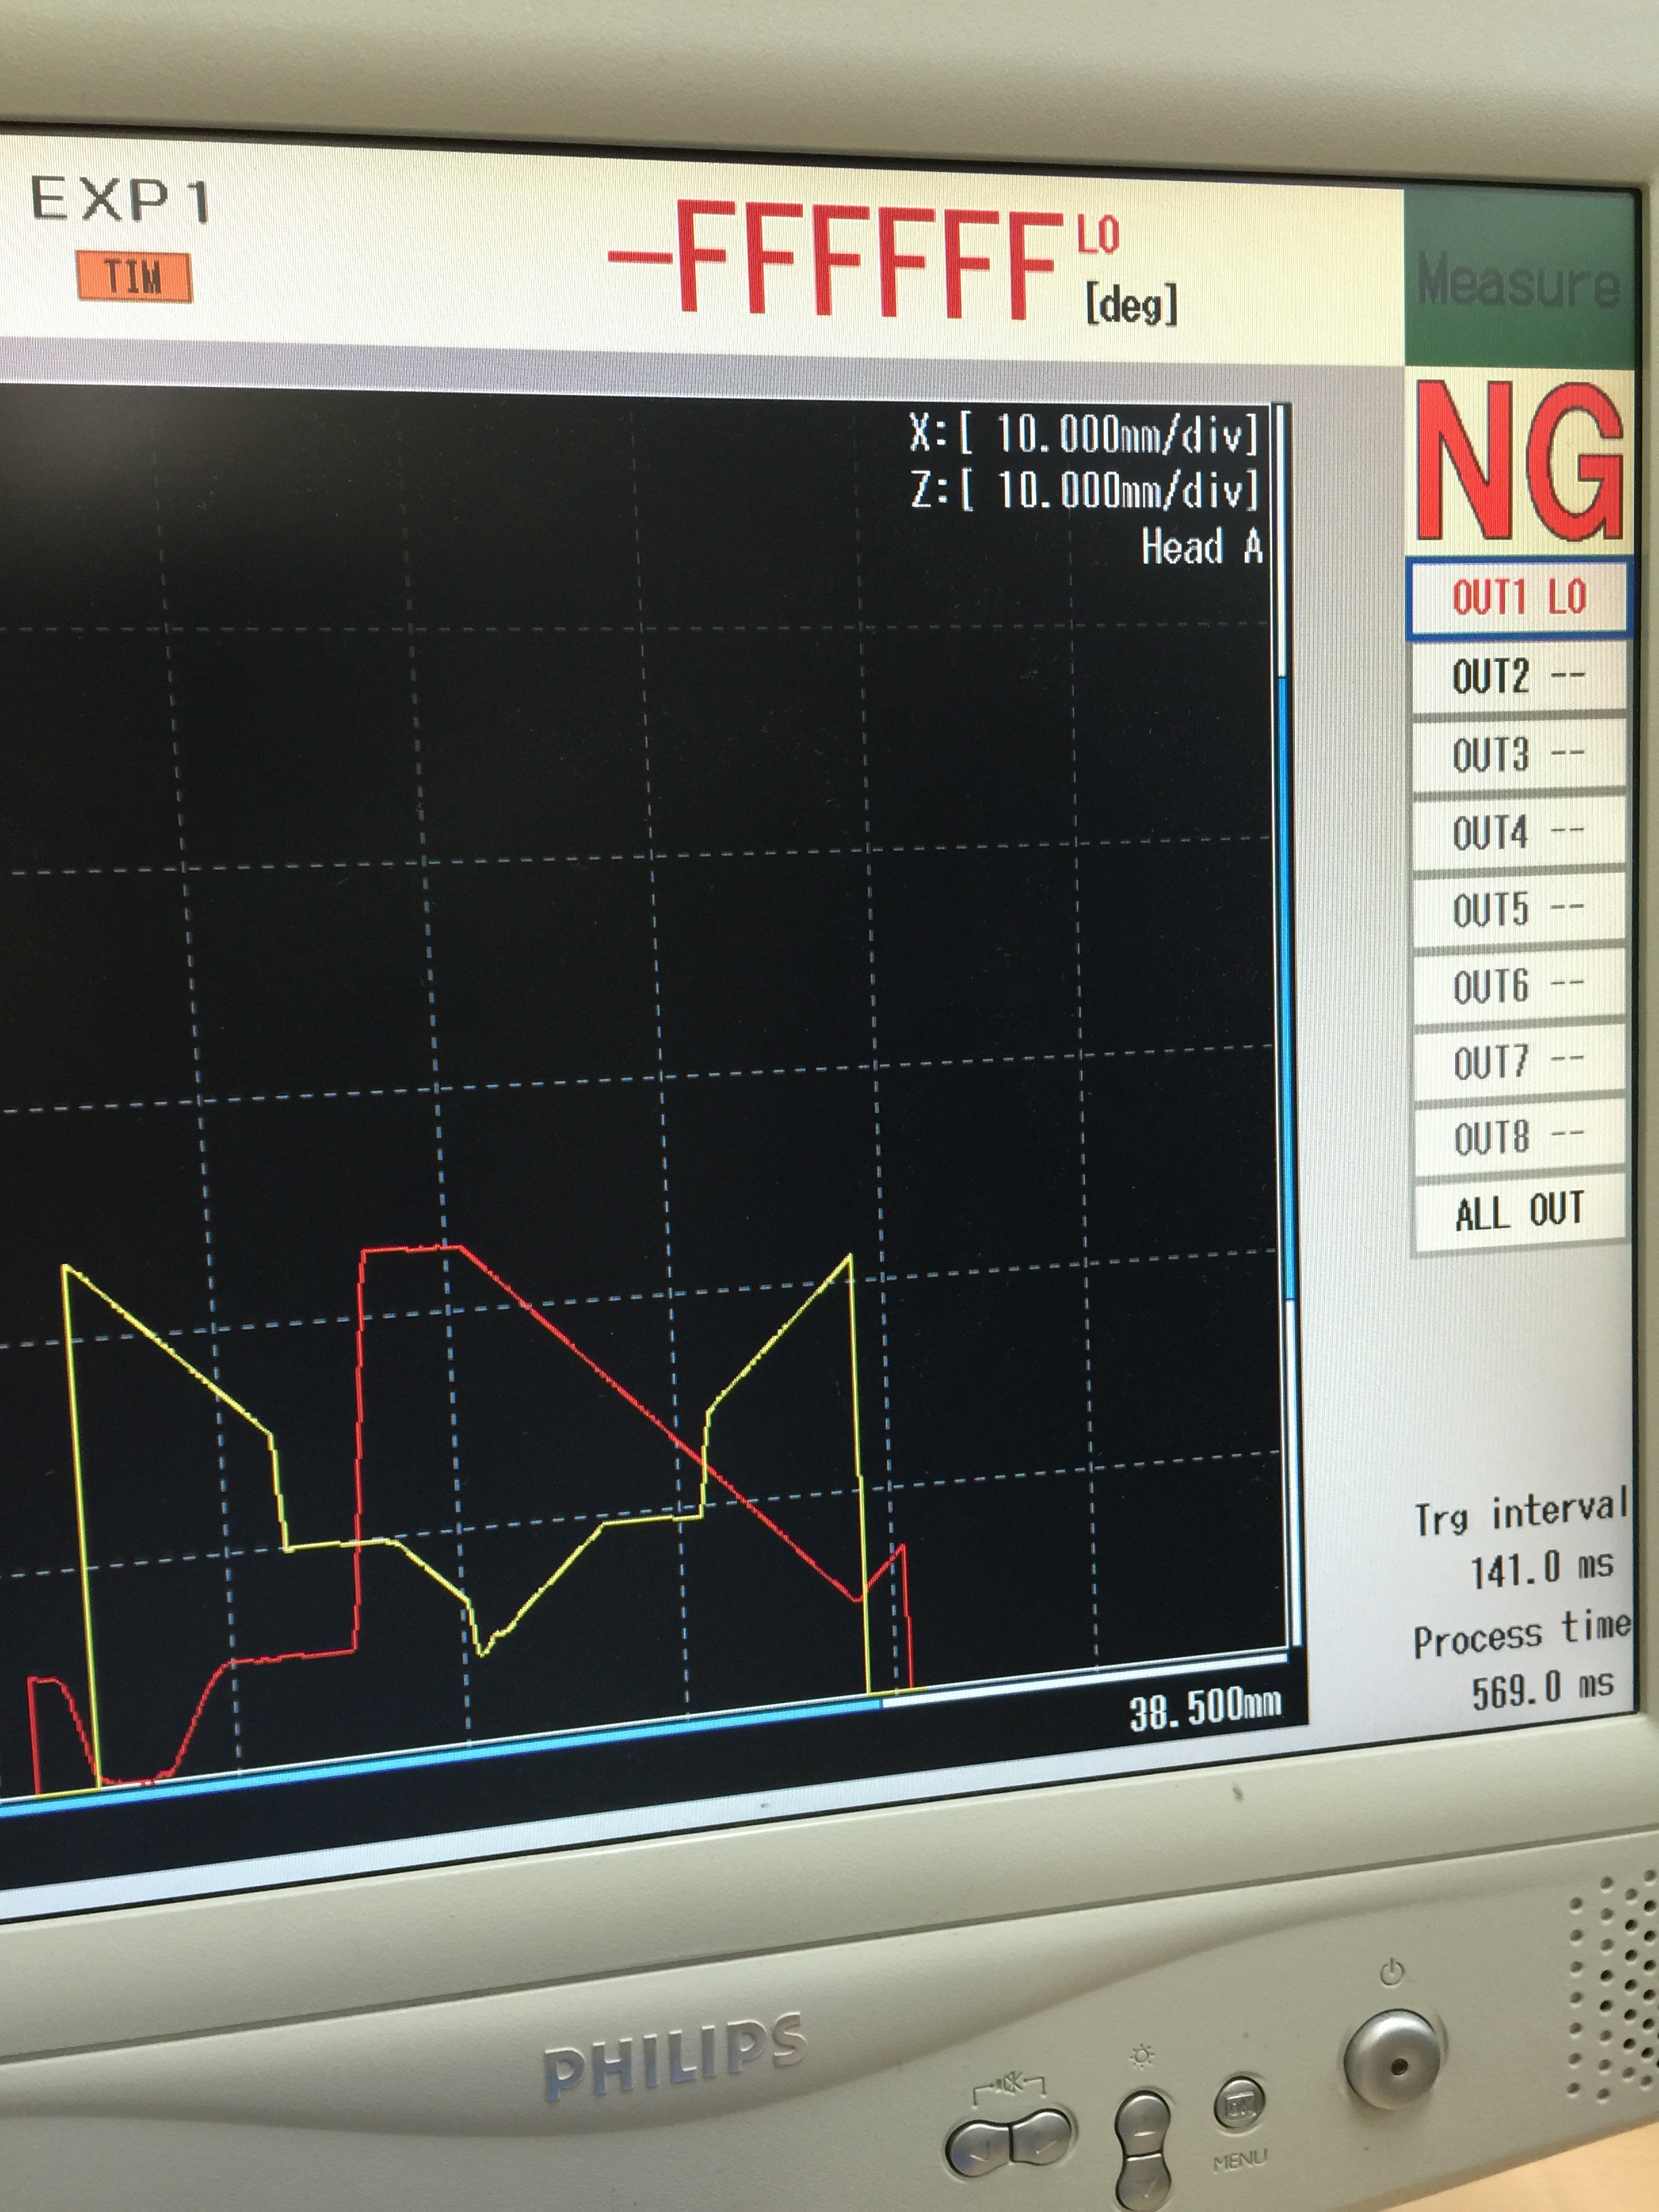
\includegraphics[width=0.45\linewidth]{Lab6/Hole2.JPG}
	}
	\caption{Hole detection}
	\label{fig:six}
\end{figure}


\section*{Conclusion}
In this experiment we used a high-accuracy laser displacement sensor with its appropriate equipment to measure and inspect physical parameters of given objects.
We used the provided software to capture the profile of the object, register it, and used it to measure the step and the angle on an object in real time. \\
We were also able to configure the laser sensor to detect the registered profile and acquire measurements even after the object has been shifted and/or rotated.\\

\section*{References}

{[}1{]} -http://www.measurecentral.com

\end{document}